%%% LaTeX Template: Article/Thesis/etc. with colored headings and special fonts
%%%
%%% Source: http://www.howtotex.com/
%%% Feel free to distribute this template, but please keep to referal to http://www.howtotex.com/ here.
%%% February 2011

%%%%% Preamble
\documentclass[10pt,a4paper]{article}
\usepackage{xspace}
\usepackage[bitstream-charter]{mathdesign}

\usepackage{textcomp} % To get get \textquotesingle

\usepackage{tikz}
\usetikzlibrary{trees}
\usetikzlibrary{arrows}
\usepackage{pgfplots}

\usepackage{environ} % For merging environments
\usepackage{framed}

%\usepackage{fancybox}


\usepackage{tgtermes}
\renewcommand*\ttdefault{txtt} % I had to include this to make the PDF output copiable
\usepackage[T1]{fontenc} % makes the characters copyable from the PDF
\usepackage[utf8]{inputenc}	
\pdfgentounicode=1

% Input encoding
\usepackage{amsmath}									% Math

\newcommand{\angstrom}{\textup{\AA}}

\usepackage{xcolor}
\definecolor{bl}{rgb}{0.0,0.2,0.6} 

\definecolor{background-image}{rgb}{1.0,0.9,0.7} 

% Translating the section, part, ... names into French
\usepackage[french]{babel}

% Setup the margins
\usepackage{geometry}

%%%%%% To get copy-pastable content of code
%https://tex.stackexchange.com/questions/62221/ensure-verbatim-code-block-is-copy-paste-able
% https://tex.stackexchange.com/questions/19949/how-to-make-listings-code-indentation-remain-unchanged-when-copied-from-pdf
\usepackage{listings}
\usepackage{textcomp}
\lstset{columns=flexible}
\lstset{keepspaces=true}
\lstset{showspaces=false}
%\makeatletter
%\def\lst@outputspace{{\ifx\lst@bkgcolor\empty\color{white}\else\lst@bkgcolor\fi\lst@visiblespace}}
%\makeatother
\lstset{
  inputencoding=utf8,
  extendedchars=true,
  literate={á}{{\'a}}1 {ã}{{\~a}}1 {é}{{\'e}}1 {è}{{\`e}}1
}
\makeatletter
\def\lst@visiblespace{ }
\makeatother
%\usepackage{listings}

\usepackage{textcomp}
\usepackage[space=true]{accsupp}

\newcommand{\pdfactualhex}[3]{\newcommand{#1}{%
\BeginAccSupp{method=hex,ActualText=#2}#3\EndAccSupp{}}}

\pdfactualhex{\pdfactualdspace}{2020}{\textperiodcentered\textperiodcentered}
\pdfactualhex{\pdfactualsquote}{27}{'}
\pdfactualhex{\pdfactualbtick}{60}{`}

\lstset{tabsize=4,basicstyle=\ttfamily,columns=flexible,emptylines=10000}
\lstset{literate={'}{\pdfactualsquote}1
                 {`}{\pdfactualbtick}1
                 {\ \ }{\pdfactualdspace}2
}

\newgeometry{margin=2cm}

% Customize the hyperlinks
\usepackage{hyperref}
\hypersetup{
    bookmarks=true,         % show bookmarks bar?
    unicode=false,          % non-Latin characters in Acrobat’s bookmarks
    pdftoolbar=true,        % show Acrobat’s toolbar?
    pdfmenubar=true,        % show Acrobat’s menu?
    pdffitwindow=false,     % window fit to page when opened
    pdfstartview={FitH},    % fits the width of the page to the window
    pdftitle={les outils du logiciel libre pour l'ingénieur},    % title
    pdfauthor={Jeremy Fix},     % author
    pdfsubject={Outils du logiciels libres pour l'ingénieur},   % subject of the document
    pdfcreator={Supélec},   % creator of the document
    pdfproducer={Producer}, % producer of the document
    pdfkeywords={keyword1} {key2} {key3}, % list of keywords
    pdfnewwindow=true,      % links in new window
    colorlinks=true,       % false: boxed links; true: colored links
    linkcolor=bl,          % color of internal links (change box color with linkbordercolor)
    citecolor=green,        % color of links to bibliography
    filecolor=magenta,      % color of file links
    urlcolor=bl           % color of external links
}

% For getting the caption on the side of an image
\usepackage{calc}
\usepackage{graphicx}
\usepackage{floatrow}
\floatsetup{style=ruled,footposition=caption}

\newcommand{\myfig}[2]{
\begin{figure}[htbp]
\floatbox[{\capbeside\thisfloatsetup{capbesideposition={right,top},capbesidewidth=4cm}}]{figure}[\FBwidth]
         {\caption{#2}\label{fig:#1}}
         {\includegraphics[width=5cm]{#1}}
\end{figure}
}


\newcommand{\question}[1]{
\textbf{Question :} #1
}
\newcommand{\indications}[0]{
\textbf{Indications :}
}

%\usepackage{sidecap}

\usepackage{sectsty}
\usepackage[compact]{titlesec} 
\allsectionsfont{\color{bl}\scshape\selectfont}

\let\LaTeXtemp\LaTeX
\newcommand{\latex}{{\Large {\LaTeXtemp\xspace} }}

%%%%% Definitions
% Define a new command that prints the title only
\makeatletter							% Begin definition
\def\printtitle{%						% Define command: \printtitle
    {\color{bl} \centering \huge \sc \textbf{\@title}\par}}		% Typesetting
\makeatother							% End definition

\title{Les outils du logiciel libre pour l'ingénieur \\ 
		\large \vspace*{-10pt} Support de cours\vspace*{10pt}}

% Define a new command that prints the author(s) only
\makeatletter							% Begin definition
\def\printauthor{%					% Define command: \printauthor
    {\centering \small \@author}}				% Typesetting
\makeatother							% End definition

\author{%
	Jérémy Fix \\
	Jeremy.Fix@CentraleSupelec.fr \\
	\vspace{20pt}
	}

% Custom headers and footers
\usepackage{fancyhdr}
	\pagestyle{fancy}					% Enabling the custom headers/footers
\usepackage{lastpage}	
	% Header (empty)
	\lhead{}
	\chead{}
	\rhead{}
	% Footer (you may change this to your own needs)
	\lfoot{\footnotesize }
	\cfoot{}
	\rfoot{\footnotesize page \thepage\ / \pageref{LastPage}}	% "Page 1 of 2"
	\renewcommand{\headrulewidth}{0.0pt}
	\renewcommand{\footrulewidth}{0.4pt}

% Change the abstract environment
\usepackage[runin]{abstract}			% runin option for a run-in title
\setlength\absleftindent{30pt}		% left margin
\setlength\absrightindent{30pt}		% right margin
\abslabeldelim{\quad}						% 
\setlength{\abstitleskip}{-10pt}
\renewcommand{\abstractname}{}
\renewcommand{\abstracttextfont}{\color{bl} \small \slshape}	% slanted text

% Pour gérer les lettrines
\usepackage{lettrine}

% Environnement Verbatim, 
\usepackage{fancyvrb}
\usepackage{color}
\usepackage{alltt}
\usepackage{upquote}

%  To be able to put verbatim within environments
\usepackage{cprotect}

\usepackage{siunitx}


% Allow linebreak in long inline equations separated by commas
\mathchardef\breakingcomma\mathcode`\,
{\catcode`,=\active
  \gdef,{\breakingcomma\discretionary{}{}{}}
}
\newcommand{\mathlist}[1]{$\mathcode`\,=\string"8000 #1$}

%% \makeatletter
%% \def\old@comma{,}
%% \catcode`\,=13
%% \def,{%
%%   \ifmmode%
%%     \old@comma\discretionary{}{}{}%
%%   \else%
%%     \old@comma%
%%   \fi%
%% }
%% \makeatother

% Some definitions

\definecolor{lgray}{gray}{0.90}
\definecolor{lblue}{RGB}{170,200,255}

\newcommand{\command}[1]{\textbf{\textit{#1}}\xspace}

\newcommand{\chemin}[1]{\textit{#1}\xspace}

\newcommand{\acroread}[0]{\command{acroread}}
\newcommand{\ant}[0]{\command{ant}}
\newcommand{\aspell}[0]{\command{aspell}}
\newcommand{\avconv}[0]{\command{avconv}}
\newcommand{\awk}[0]{\command{awk}}
\newcommand{\basename}[0]{\command{basename}}
\newcommand{\bashcmd}[0]{\command{bash}}
\newcommand{\bibtex}[0]{\command{bibtex}}
\newcommand{\cat}[0]{\command{cat}}
\newcommand{\cd}[0]{\command{cd}}
\newcommand{\convert}[0]{\command{convert}}
\newcommand{\cut}[0]{\command{cut}}
\newcommand{\cmake}[0]{\command{cmake}}
\newcommand{\diff}[0]{\command{diff}}
\newcommand{\du}[0]{\command{du}}
\newcommand{\echo}[0]{\command{echo}}
\newcommand{\egrep}[0]{\command{egrep}}
\newcommand{\emacs}[0]{\command{emacs}}
\newcommand{\evince}[0]{\command{evince}}
\newcommand{\find}[0]{\command{find}}
\newcommand{\ffmpeg}[0]{\command{ffmpeg}}
\newcommand{\gawk}[0]{\command{gawk}}
\newcommand{\gimp}[0]{\command{Gimp}}
\newcommand{\graphicsmagick}[0]{\command{GraphicsMagick}}
\newcommand{\grep}[0]{\command{grep}}
\newcommand{\gzip}[0]{\command{gzip}}
\newcommand{\head}[0]{\command{head}}
\newcommand{\hunspell}[0]{\command{hunspell}}
\newcommand{\imagemagick}[0]{\command{ImageMagick}}
\newcommand{\ispell}[0]{\command{ispell}}
\newcommand{\join}[0]{\command{join}}
\newcommand{\less}[0]{\command{less}}
\newcommand{\ls}[0]{\command{ls}}
\newcommand{\LanguageTool}[0]{\command{LanguageTool}}
\newcommand{\locate}[0]{\command{locate}}
\newcommand{\lynx}[0]{\command{lynx}}
\newcommand{\make}[0]{\command{make}}
\newcommand{\makefile}[0]{\command{makefile}}
\newcommand{\man}[0]{\command{man}}
\newcommand{\matplotlib}[0]{\command{matplotlib}}
\newcommand{\mencoder}[0]{\command{mencoder}}
\newcommand{\mkdir}[0]{\command{mkdir}}
\newcommand{\mplayer}[0]{\command{mplayer}}
\newcommand{\myspell}[0]{\command{myspell}}
\newcommand{\numpy}[0]{\command{numpy}}
\newcommand{\okular}[0]{\command{okular}}
\newcommand{\pdflatex}[0]{\command{pdflatex}}
\newcommand{\pdftk}[0]{\command{pdftk}}
\newcommand{\python}[0]{\command{python}}
\newcommand{\pwd}[0]{\command{pwd}}
\newcommand{\qmake}[0]{\command{qmake}}
\newcommand{\readcmd}[0]{\command{read}}
\newcommand{\recordMyDesktop}[0]{\command{recordmydesktop}}
\newcommand{\myrm}[0]{\command{rm}}
\newcommand{\shutter}[0]{\command{shutter}}
\newcommand{\scons}[0]{\command{scons}}
\newcommand{\sed}[0]{\command{sed}}
\newcommand{\sort}[0]{\command{sort}}
\newcommand{\tail}[0]{\command{tail}}
\newcommand{\tar}[0]{\command{tar}}
\newcommand{\UnetBootin}[0]{\command{unetbootin}}
\newcommand{\unzip}[0]{\command{unzip}}
\newcommand{\updatedb}[0]{\command{updatedb}}
\newcommand{\wget}[0]{\command{wget}}
\newcommand{\xfig}[0]{\command{xfig}}
\newcommand{\zenity}[0]{\command{Zenity}}
\newcommand{\zip}[0]{\command{zip}}
\newcommand{\zmore}[0]{\command{zmore}}
\newcommand{\zgrep}[0]{\command{zgrep}}

%%\newcommand{\bash}[1]{{\texttt{#1}}}
%\newcommand{\bash}[1]{{\verb+#1}}
\newcommand{\bash}[1]{{\ttfamily #1}}

\newcommand{\todo}[0]{\textbf{!!!todo!!!}}


%\newcommand{\dollar}[0]{$}

\newcommand{\encadreUtilisation}[1]{
\noindent\fcolorbox{black}{lgray}{
\begin{minipage}{\columnwidth}
#1
\end{minipage}
}
}

% Pour les TP
\newcommand{\datesoleil}[0]{31 août 2012\xspace}
\newcommand{\lambdasoleil}[0]{211 \si{\AA}\xspace}
\newcommand{\urlsoleil}[0]{\url{http://jsoc.stanford.edu/data/aia/images}\xspace}

\newenvironment{exempleResultat}{
\VerbatimEnvironment 
\begin{framed}
\begin{center}
\begin{footnotesize}
\begin{alltt}
}
{
\end{alltt}
\end{footnotesize}
\end{center}
\end{framed}
}

% Defines a `datastore' shape for use in DFDs.  This inherits from a
% rectangle and only draws two horizontal lines.
\makeatletter
\pgfdeclareshape{datastore}{
  \inheritsavedanchors[from=rectangle]
  \inheritanchorborder[from=rectangle]
  \inheritanchor[from=rectangle]{center}
  \inheritanchor[from=rectangle]{base}
  \inheritanchor[from=rectangle]{north}
  \inheritanchor[from=rectangle]{north east}
  \inheritanchor[from=rectangle]{east}
  \inheritanchor[from=rectangle]{south east}
  \inheritanchor[from=rectangle]{south}
  \inheritanchor[from=rectangle]{south west}
  \inheritanchor[from=rectangle]{west}
  \inheritanchor[from=rectangle]{north west}
  \backgroundpath{
    %  store lower right in xa/ya and upper right in xb/yb
    \southwest \pgf@xa=\pgf@x \pgf@ya=\pgf@y
    \northeast \pgf@xb=\pgf@x \pgf@yb=\pgf@y
    \pgfpathmoveto{\pgfpoint{\pgf@xa}{\pgf@ya}}
    \pgfpathlineto{\pgfpoint{\pgf@xb}{\pgf@ya}}
    \pgfpathmoveto{\pgfpoint{\pgf@xa}{\pgf@yb}}
    \pgfpathlineto{\pgfpoint{\pgf@xb}{\pgf@yb}}
 }
}
\makeatother


%%%%%%%%%%%%%%%%%%%%%%%%%%%%%%%%%%%%%%%%%%%%%%%%%%%%%%%%%%%%%%%%%%%%%%%%%%
%%% Start of the document
%%%%%%%%%%%%%%%%%%%%%%%%%%%%%%%%%%%%%%%%%%%%%%%%%%%%%%%%%%%%%%%%%%%%%%%%%%
\begin{document}
%%% Top of the page: Author, Title and Abstact
\printtitle 

\printauthor

\begin{abstract}
On décrit dans ce document un ensemble d'outils libres permettant de
résoudre notamment des problèmes que des ingénieurs seront amenés à
rencontrer. Ce document peut être considéré comme une boite à outils
avec un ensemble de références et d'exemples d'utilisation de
logiciels libres. Il a pour but d'avoir un aspect pratique en ne se
focalisant que sur quelques exemples d'utilisation de ces logiciels
sans en faire une description exhaustive.
\end{abstract}

\tableofcontents

%% \pagebreak
%% \part{Introduction au logiciel libre}

%% Introduction à Unix, les différentes distributions vite fait, la
%% notion de licence (BSD, Creative commons, BSD, GPL, ...)\\

%% \url{http://fr.slideshare.net/eurolinux/introduction-aux-logiciels-libres-2459812}

\pagebreak

\part{Familiarisation avec l'environnement Unix}

Il existe un très grand nombre de distributions linux, vous en trouverez quelques unes mentionnées sur le site distrowatch \url{http://distrowatch.com/dwres.php?resource=major}. Nous allons nous intéresser uniquement aux distributions Fedora (la distribution installée sur les machines de l'école) et Ubuntu. 

%Sur le site du zéro: \url{http://fr.openclassrooms.com/informatique/cours/reprenez-le-controle-a-l-aide-de-linux}

%% \section{Distribution Ubuntu}

%% Il existe un grand nombre de distributions Linux, les plus populaires étant Ubuntu et Fedora (\todo). Les développeurs de Fedora produisent également une version payante RedHat. Cette version payante est ... ; 

%% Dans ce cours, nous allons utiliser Ubuntu.  

\section{En route pour Linux: Live CD/USB}
\label{sec:unetbootin}

La plupart des distributions Linux peuvent être exécutées à partir d'une clef USB, ce qui fait qu'il est extrêmement simple de tester une distribution de manière non invasive. Certaines de ces distributions, comme Ubuntu, autorisent également un espace de stockage permanent sur la cle. Si vous installez des logiciels depuis votre Ubuntu USB, ces logiciels seront toujours installés lorsque vous aurez redémarré votre PC. Pour créer une clé USB bootable, vous pouvez utiliser le logiciel \UnetBootin. Il est téléchargeable pour différentes plateformes à l'adresse \url{http://unetbootin.sourceforge.net/}. Vous devez disposer d'une clé USB formattée en fat-32. Les figures~\ref{fig:unetbootin} illustrent quelques copies d'écran d'unetbootin utilisé pour créer une live USB d'Ubuntu.

\begin{figure}[htbp]
\begin{tabular}{ccc}
\includegraphics[width=0.3\columnwidth]{Figs/unetbootin1.png}&
\includegraphics[width=0.3\columnwidth]{Figs/unetbootin2.png}&
\includegraphics[width=0.3\columnwidth]{Figs/unetbootin3.png}\\
a) & b) & c)
\end{tabular}
\caption{\label{fig:unetbootin} a) Unetbootin une fois lancé; b) On commence par sélectionner la distribution pour laquelle créer une live USB, ici Ubuntu 12.04 Live; c) On précise l'emplacement de la clé USB et l'espace permanent à réserver. Et c'est fini.}
\end{figure}

Une fois que la clé est créée, il vous suffit de redémarrer la machine en indiquant au BIOS de booter en priorité sur la clé USB (surtout, avant le disque dur). Vous arrivez donc sur le bureau Unity (fig.~\ref{fig:ubuntu_live}). Vous pouvez tester Ubuntu, tout sera sauvegardé sur l'espace permanent de la clé USB. 

\begin{figure}[htbp]
\includegraphics[width=0.5\columnwidth]{Figs/ubuntu_12_04_live.png}
\caption{\label{fig:ubuntu_live} Votre premier contact avec Ubuntu 12.04}
\end{figure}


%% \subsection{Système de fichier}

%% L'organisation des fichiers ..


%% Pour naviguer dans le système de fichier, on utilisera les commandes $cd, pwd, ls$. 

%% \subsection{Utilisateurs, groupes et permissions}
%% \label{sec:permissions}
%% Chaque utilisateur est identifié par un login, disons \emph{toto}, et dispose d'un espace personnel accessible à \chemin{/home/toto}. Il appartient également au groupe \emph{toto}. Par défaut, un utilisateur n'appartient qu'au groupe qui porte son nom. Il est possible et même fréquent qu'un utilisateur appartiennent à plusieurs groupes; par exemple, un groupe correspond aux personnes ayant le droit d'administrer les imprimantes, un autre groupe correspond aux personnes ayant le droit d'administrer le système, ... . Il existe un utilisateur particulier, \emph{root}, qui a les droits \todo.\\





%% \subsection{Gestion de packages}

%% voir par exemple comment installer des paquets, et comment l'inclure
%% dans la suite du document...

%% \subsection{Obtenir des informations sur une commande}

%% man page, info ou parfois simplement exécuter le binaire et un message
%% d'aide s'affiche, ou binaire --help ou binaire -h

\pagebreak
\part{Outils pour la manipulation et l'édition de fichiers}

%% \section{TODO}
%% \begin{itemize}
%% \item Astuce pour vérifier l'orthographe de plusieurs fichiers : \bash{find
%%   . -name "*.tex" -exec aspell --lang=en --mode=tex check "{}" \;}
%% \item les redirections avec les pipes
%% \item diff, man ,...
%% \item doxygen
%% \item django, .. des frameworks pour le web
%% \item pour egrep: \url{http://www-etud.iro.umontreal.ca/~tsikhana/IFT1215-H11/files/Unix3.pdf}
%% \end{itemize}

\section{Les outils GNU}

Dans les prochaines sections, on verra un certain nombre de programme. Certains d'entre sont des outils GNU dont la philosophie est décrite dans le manuel \bash{info coreutils 'Toolbox Introduction'}. Cette description est rappelée ci-dessous;

This month's column is only peripherally related to the GNU Project, in
that it describes a number of the GNU tools on your GNU/Linux system
and how they might be used.  What it's really about is the "Software
Tools" philosophy of program development and usage.

   The software tools philosophy was an important and integral concept
in the initial design and development of Unix (of which Linux and GNU
are essentially clones).  Unfortunately, in the modern day press of
Internetworking and flashy GUIs, it seems to have fallen by the
wayside.  This is a shame, since it provides a powerful mental model
for solving many kinds of problems.

   Many people carry a Swiss Army knife around in their pants pockets
(or purse).  A Swiss Army knife is a handy tool to have: it has several
knife blades, a screwdriver, tweezers, toothpick, nail file, corkscrew,
and perhaps a number of other things on it.  For the everyday, small
miscellaneous jobs where you need a simple, general purpose tool, it's
just the thing.

   On the other hand, an experienced carpenter doesn't build a house
using a Swiss Army knife.  Instead, he has a toolbox chock full of
specialized tools--a saw, a hammer, a screwdriver, a plane, and so on.
And he knows exactly when and where to use each tool; you won't catch
him hammering nails with the handle of his screwdriver.

   The Unix developers at Bell Labs were all professional programmers
and trained computer scientists.  They had found that while a
one-size-fits-all program might appeal to a user because there's only
one program to use, in practice such programs are

  a. difficult to write,

  b. difficult to maintain and debug, and

  c. difficult to extend to meet new situations.

   Instead, they felt that programs should be specialized tools.  In
short, each program "should do one thing well."  No more and no less.
Such programs are simpler to design, write, and get right--they only do
one thing.

   Furthermore, they found that with the right machinery for hooking
programs together, that the whole was greater than the sum of the
parts.  By combining several special purpose programs, you could
accomplish a specific task that none of the programs was designed for,
and accomplish it much more quickly and easily than if you had to write a special purpose program.  We will see some (classic) examples of this
further on in the column.  (An important additional point was that, if
necessary, take a detour and build any software tools you may need
first, if you don't already have something appropriate in the toolbox.)

\section{Éditeur de texte emacs}
\label{sec:emacs}

GNU Emacs\footnote{\url{http://www.gnu.org/software/emacs/}} est un
éditeur de texte très largement personnalisable. Il dispose notamment
d'un grand nombre de \emph{mode} chargé automatiquement en fonction de
l'extension du fichier édité. Il existe par exemple des modes Python,
C++, C, CamL, HTML, ... Ces modes introduisent les colorations
syntaxiques et indentations spécifiques aux langages ainsi que des
outils en personnalisant la barre des menus. Les figures~\ref{fig:emacs_python.eps},\ref{fig:emacs_cpp.eps} montrent
des exemples d'emacs éditant un fichier Python et un fichier C++. On
pourra remarquer qu'en fonction du fichier édité, la barre de menu est
différente.\\

\begin{figure}[htbp]
\begin{floatrow}[2]
\ffigbox[.5\FBwidth]{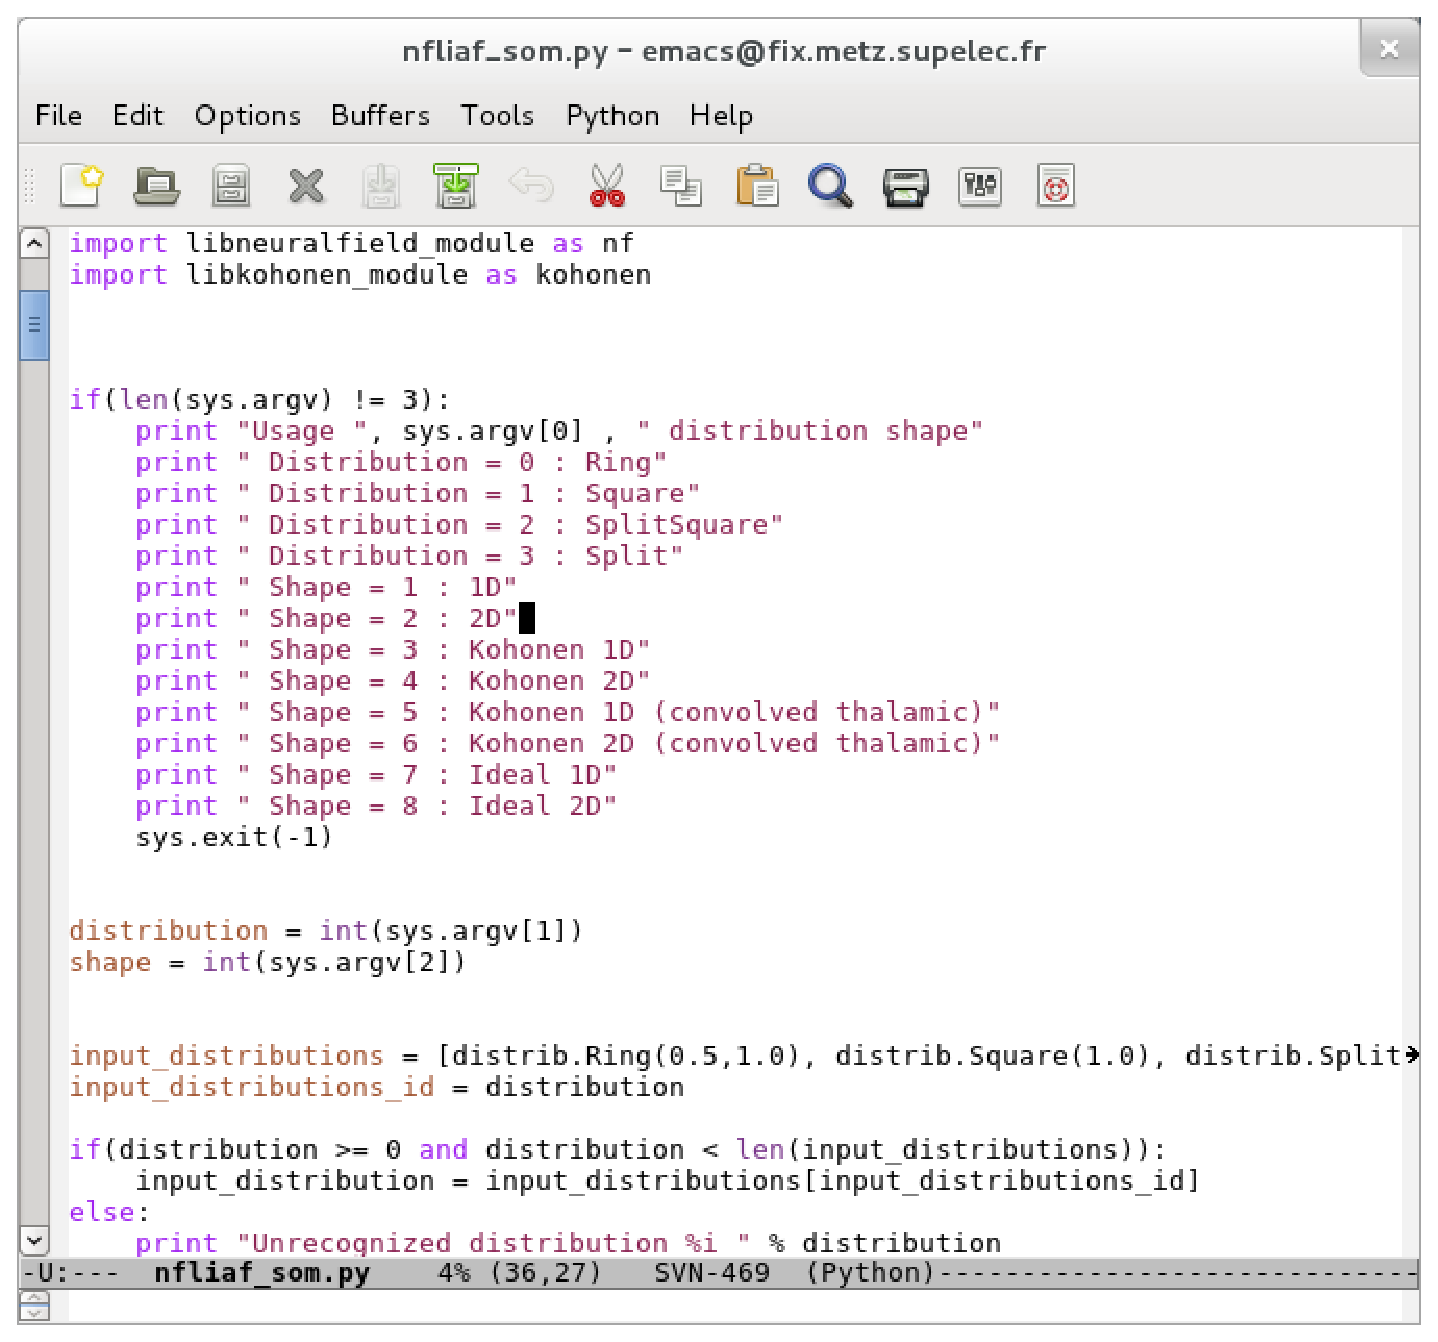
\includegraphics[width=\columnwidth]{Figs/emacs_python.eps}}{\caption{Emacs
  utilisé pour éditer un fichier Python}\label{fig:emacs_python.eps}}
\ffigbox[.5\FBwidth]{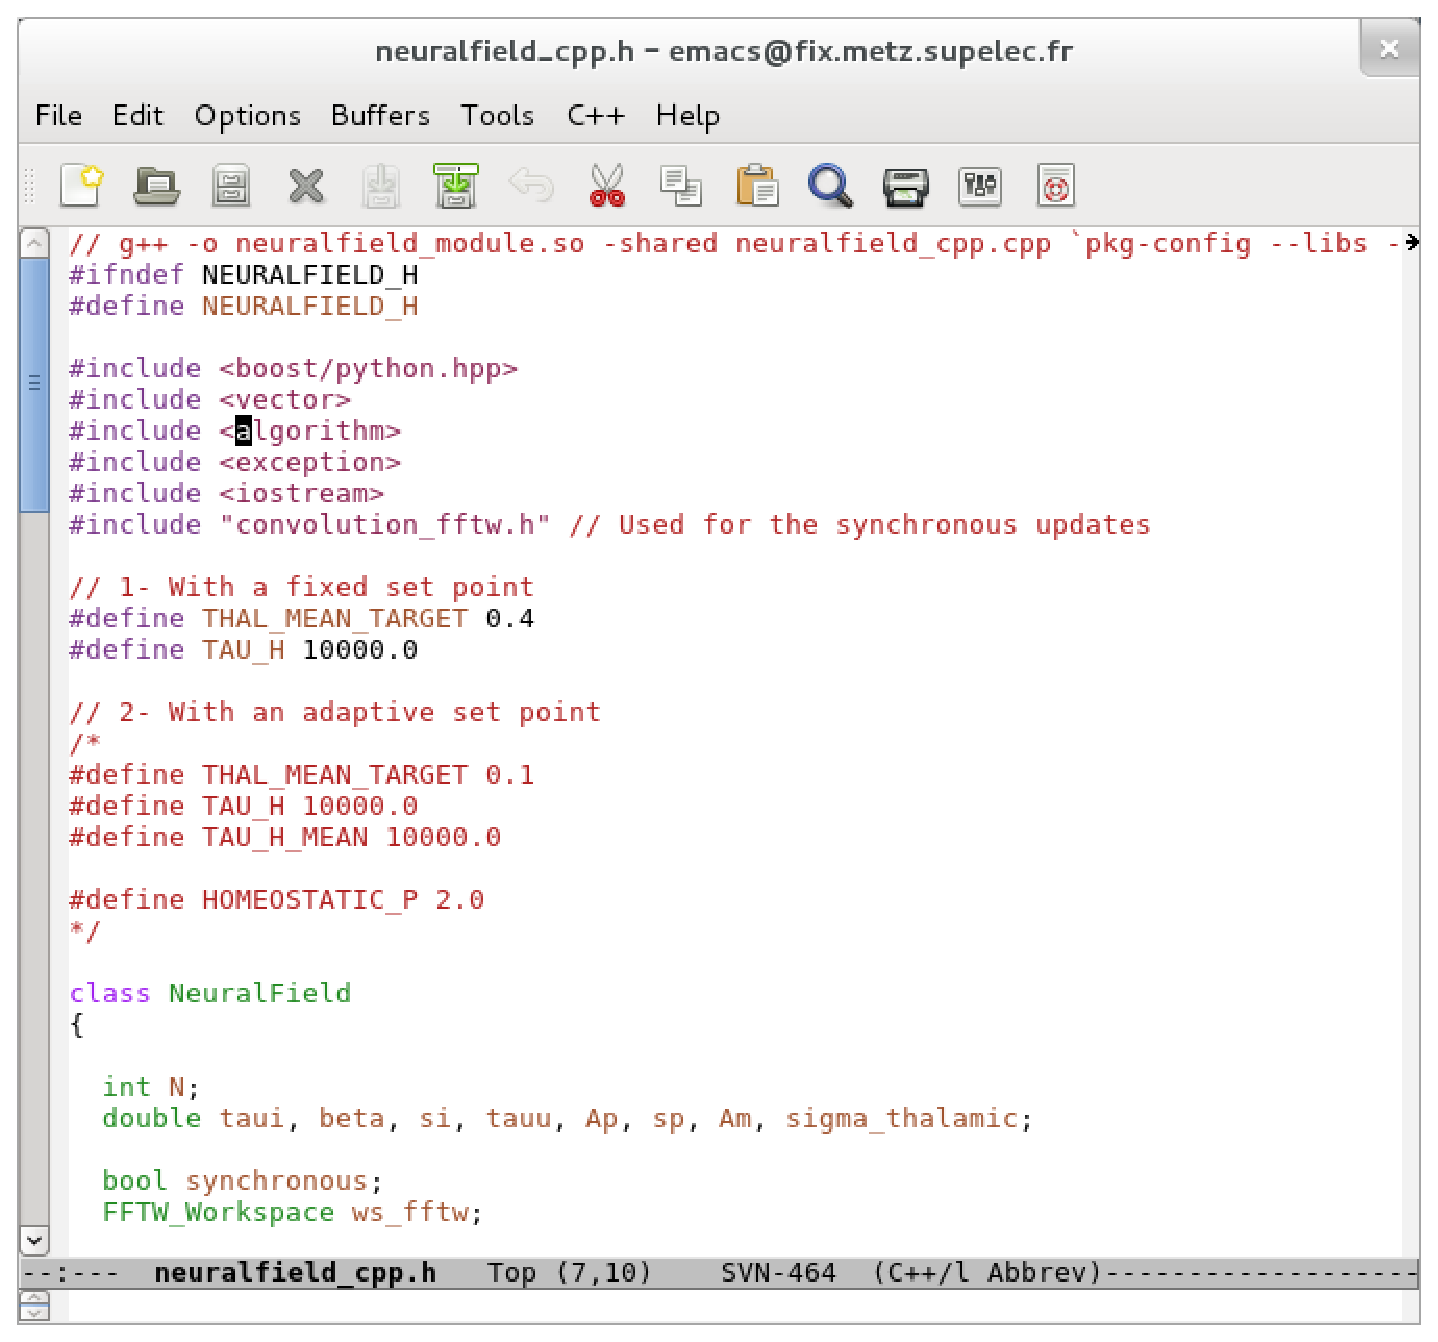
\includegraphics[width=\columnwidth]{Figs/emacs_cpp.eps}}{\caption{Emacs
  utilisé pour éditer un fichier C++}\label{fig:emacs_cpp.eps}}
\end{floatrow}
\end{figure}

Emacs peut paraître un peu austère mais il s'avère extrêmement
pratique à partir du moment o{\`u} on connaît un certain nombre de
raccourcis clavier. Utiliser ces raccourcis clavier est un peu
fastidieux au début mais devient rapidement un automatisme très
confortable\footnote{Rappelez vous quand vous avez appris à faire du
  vélo}. \textbf{Attention}: on indiquera un raccourcis comme
\emph{\underline{Ctrl} - X - F} pour indiquer qu'il faut presser sur
la touche Ctrl du clavier, la \underline{maintenir} enfoncée puis
presser successivement les touches X et F. Lorsqu'on lance un
raccourci, des informations peuvent être affichées dans la zone de
texte tout en bas de l'éditeur. Voici une liste de
raccourcis utiles~:\\
\begin{tabular}{cl}
 \underline{Ctrl} - G &: Annuler la commande en cours\\
 \underline{Ctrl} - X - F &: Ouvrir un fichier existant ou le
  créer\\
 \underline{Ctrl} - \_ &: Annuler la dernière commande\\
 \underline{Ctrl} - X - S &: Sauvegarder un fichier\\
 \underline{Ctrl} - K &: Supprimer la ligne courante à partir du
  curseur\\
 \underline{Ctrl} - W &: Supprimer la sélection\\
 \underline{Ctrl} - X puis H &: sélectionner tout le texte du
  buffer courant \\
&(pratique si on poursuit par Tab pour indenter tous
  le buffer d'un coup)\\
\underline{Tab} &: Indente la sélection (en fonction du mode courant)\\
 \underline{Ctrl} - S &: Rechercher dans le fichier ouvert\\
 \underline{Shift} - \underline{Alt} - \% &: Rechercher/Remplacer\\
 \underline{Ctrl} - X puis \underline{Shift} - 1 &: Définir la
  disposition des fenêtre pour n'éditer qu'un buffer à la foi\\
& (voir
  les deux prochains raccourcis pour mieux comprendre!)\\
 \underline{Ctrl} - X puis \underline{Shift} - 2 &: Diviser en deux la
  fenêtre d'édition verticalement\\
 \underline{Ctrl} - X puis \underline{Shift} - 3 &: Diviser en deux la
  fenêtre d'édition horizontalement\\
 \underline{Alt} - X &: Saisir directement une commande dans la
  zone de texte en bas de l'éditeur\\
\end{tabular}


Cette dernière commande qui se lit ``Meta-X'' permet d'accéder à la
zone de texte sous l'éditeur (mini-buffer) et dans laquelle on peut saisir des
commandes comme~:
\begin{itemize}
\item goto-line : suivie d'entrée, elle permet de saisir une ligne à
  laquelle se rendre (pratique si la compilation d'un fichier échoue
  et qu'un numéro de ligne o{\`u} se trouve l'erreur est mentionné
\item comment-region : commente la sélection
\item uncomment-region : décommente la sélection
\item ispell-change-dictionnary : pour changer le dictionnaire utilisé
  pour la correction orthographique en ligne
\item flyspell-buffer : pour lancer le correcteur orthographique sur
  tous le buffer courant
\item flyspell-mode : pour activer/désactiver la correction
  orthographique à la volée
\item c++-mode : basculer en mode C++ (pour la coloration syntaxique,
  l'indentation, etc...)
\item python-mode : basculer en mode Python (pour la coloration syntaxique,
  l'indentation, etc...)
\item tuareg-mode : basculer en mode CamL (pour la coloration syntaxique,
  l'indentation, etc...)
\item octave-mode : basculer en mode Octave (pour la coloration syntaxique,
  l'indentation, etc...)
\end{itemize}

N'oubliez pas que dans le monde Unix, la tabulation permet
d'auto-compléter une commande. Par exemple, pour la commande
\emph{uncomment-region}, il suffira de saisir \emph{unc} suivi de
Tabulation pour que la commande soit complétée. Si plusieurs commandes
ont le même préfixe, une liste des choix s'affiche si on appuis deux
fois sur tabulation.\\


Revenons quelques instants sur la notion de mode dans \emacs. \emacs
est écrit pour être modulable et adaptable à ses besoins (plus besoin
d'un éditeur spécifique pour éditer du texte, du latex, du C++,
... \emacs se spécialise en fonction de l'extension du fichier édité). Les modes
pour \emacs introduisent justement cette flexibilité. On parlait plus
haut des modes c++, python, tuareg qui modifient les menus de
l'éditeur, les raccourcis claviers, l'indentation, la coloration
syntaxique. Ces modes sont appelés \textbf{modes majeurs}. Il en
existe plusieurs pour les langages de programmation les plus répandus
(\url{http://fr.wikipedia.org/wiki/Emacs}). En pratique, ces modes
sont écrits comme des scripts Lisp. Il est également possible de
personnaliser l'interface à l'aide de scripts Lisp.\\

Pour la correction orthographique, il peut falloir installer des
packages supplémentaires. Nous verrons dans la prochaine partie
quelques outils qui permettent une correction orthographique à la
volée et qui disposent de modes \emacs.\\

Enfin, il existe des alternatives à \emacs mais que je trouve trop
spécifique ou moins pratique d'utilisation qu'\emacs: gedit,
LibreOffice, Kate, ... . Même si Libreoffice propose plus que de
l'édition de texte, on verra plus tard des alternatives que je préfère
(Latex pour produire des documents textuels, beamer pour faire des
supports de présentation, python/matplotlib pour tracer des données).

\section{Correction orthographique/grammaticale}
\label{sec:correction_orthographique}

Il existe un certain nombre de logiciels libres pour la correction
orthographique et/ou grammaticale, notamment \ispell, \aspell,
\myspell, \hunspell, \LanguageTool, ... . L'historique des différentes
versions xxxspell n'est pas très clair. \ispell semble être le plus
ancien, sur lequel est basé \myspell; \aspell semble avoir été
développé pour prendre le relais d'\ispell. \hunspell quand à lui est
le correcteur orthographique qui semble prendre la main; Il est
utilisé dans un grand nombre d'applications comme Firefox,
Thunderbird, Chrome, Eclipse, ...\footnote{Plus d'informations sont
  disponibles sur la page
  \url{http://en.wikipedia.org/wiki/Hunspell}}. \LanguageTool semble
avoir été développé plus récemment et indépendemment. Contrairement
aux xxx-spell, LanguageTool corrige les formes de style évitant ainsi,
par exemple, l'utilisation de pléonasmes (au jour d'aujourd'hui),
l'utilisation de deux virgules consécutives, etc. .\\

Pour installer ces logiciels (on préférera \aspell, \hunspell ou
\LanguageTool) sous Fedora :\\
\begin{itemize}
\item Aspell : \bash{yum install aspell aspell-fr aspell-en}, les
  paquets aspell-fr aspell-en étant les dictionnaires français et
  anglais,
\item Hunspell : \bash{yum install hunspell hunspell-fr hunspell-en},
  les paquets hunspell-fr hunspell-en étant les dictionnaires français
  et anglais,
\item LanguageTool : il faut aller chercher l'archive java fournis sur
  le site : \url{http://www.languagetool.org/}
\end{itemize}

Tout ces outils sont utilisables en ligne de commande (i.e. dans un
terminal, depuis un Makefile, ...). Pour tester les possibilités des
différents correcteurs, on partira du texte ci-dessous, les fautes
étant indiquées en rouge~:

\begin{center}
\fbox{\begin{minipage}{0.5\textwidth}
Maître Corbeau, sur un arbre \textcolor{red}{perchai},\\
\textcolor{red}{Tenais} en son \textcolor{red}{beck} un fromage.\\
Maître Renard, par l'odeur alléché,\\
Lui tint à peu près ce langage :\\
"Hé ! bonjour, Monsieur du Corbeau.\\
Que vous êtes joli ! que vous me semblez beau !\\
Sans mentir, si votre ramage\\
Se rapporte à votre plumage,\\
Vous êtes le Phénix des hôtes de ces bois. "\\
A ces mots le Corbeau ne se sent pas de joie ;\\
Et pour montrer sa belle voix,\\
Il ouvre un large bec, laisse tomber sa proie.\\
Le Renard s'en \textcolor{red}{saisie}, et dis : "Mon bon Monsieur,\\
\textcolor{red}{Apprené} que tout flatteur\\
Vit aux dépens de celui qui l'écoute :\\
Cette leçon vaut bien un fromage, sans doute. "\\
Le Corbeau, honteux et confus,\\
Jura, mais un peu tard, qu'on ne l'y prendrait plus.
\end{minipage}}
\end{center}

\encadreUtilisation{
\textbf{Utilisation d'Aspell}:\\

\aspell s'appelle avec une commande de la forme :\\
\centerline{\bash{aspell check [options] filename}}\\
\noindent Plusieurs options sont disponibles, on ne liste que les plus utiles\footnote{les autres sont documentées sur la page \url{http://aspell.net/man-html/Spellchecking-Individual-Files.html\#Spellchecking-Individual-Files} }:
\begin{itemize}
\item \bash{-{}-lang=name}, avec name $\in$ \{fr, en, ..\} permet de spécifier le language
\item \bash{-{}-mode=mode}, avec mode $\in$ \{none, url, email, sgml, tex, texinfo, nroff, ..\} permet de filtrer des mots clefs spécifiques de language (par exemple, le mode tex permet de ne pas considérer les mots clefs \LaTeX)
\end{itemize}

\noindent Pour avoir plus d'informations sur les options à passer au programme,
on utilisera~:
\begin{center}
\bash{aspell -{}-help}
\end{center}

\noindent Par exemple, pour corriger les fautes d'orthographes d'un fichier
texte, on utilisera:
\begin{center}
\bash{aspell check -lfr text.txt}
\end{center}
\noindent pour corriger les fautes d'orthographes d'un fichier
\LaTeX, on utilisera:
\begin{center}
\bash{aspell check -lfr -{}-mode=tex text.tex}
\end{center}
Ces deux commandes lancent aspell en mode intéractif, permettant de
corriger les fautes à la volée (le fichier original est modifié). On
peut aussi lister les fautes, sans les corriger. Sur le texte de Jean
de la Fontaine, \aspell retourne~:\\
\bash{more original.txt | aspell -lfr list}\\
\indent \indent beck\\
\indent \indent Apprené\\
}

\encadreUtilisation{ \textbf{Utilisation d'Hunspell}:\\ 

\hunspell
  fonctionne de manière similaire à \aspell, les options étant
  spécifiées de manière un peu différente. Pour avoir plus
  d'informations sur les options à passer au programme, on utilisera~:
\begin{center}
\bash{hunspell --help}
\end{center} 
\noindent Pour vérifier l'orthographe
d'un texte en Français, on utilisera la commande~:
\begin{center}
\bash{hunspell -d fr\_FR text.txt}
\end{center}
Pour vérifier un document \LaTeX, on précisera l'option \bash{-t}~:
\begin{center}
\bash{hunspell -d fr\_FR -t text.tex}
\end{center}
 On peut aussi lister les fautes, sans les corriger. Sur le texte de Jean
de la Fontaine, \hunspell retourne~:\\
\bash{hunspell -d fr\_FR -l original.txt}\\
\indent \indent beck\\
\indent \indent Apprené\\
}

\encadreUtilisation{ \textbf{Intégration dans \emacs}:\\ 
\aspell et \hunspell peuvent être intégrés à \emacs pour avoir une
correction orthographique à la volée. Comme nous l'avons vu dans la
partie sur \emacs, on peut le personnaliser en ajoutant des commandes
Lisp au fichier \bash{~/.emacs}. Pour indiquer qu'on souhaite utiliser
aspell pour vérifier l'orthographe, on ajoutera la commande~:
\begin{center}
\bash{(setq-default ispell-program-name "aspell")}
\end{center}
On utilisera alors la correction orthographique avec les commandes
ci-dessous, à exécuter dans le mini-buffer(``Meta-X'', \underline{Alt} - X)
\begin{itemize}
\item ispell-change-dictionnary , suivi de fr ou en par exemple :
  change le dictionnaire courant
\item flyspell-buffer : vérifie l'orthographe du fichier en cours d'édition
\item flyspell-mode : active/désactive la correction à la volée
\end{itemize}
On fera bien attention que lorsque le dictionnaire est changé, il faut
relancer la commande \bash{flyspell-buffer} pour le prendre en compte.
}


\section{Automatisation de tâches avec Makefile}
\label{sec:makefile}

On a vu et on verra des commandes à exécuter dans un terminal pour
résoudre un certain nombre de problèmes (vérifier l'orthographe d'un
texte, travailler des images, regrouper des images pour créer une
vidéo, lister/modifier un ensemble de fichiers, compiler un document
\LaTeX, compiler un programme, ...). Il peut devenir difficile de se souvenir de la syntaxe
d'une commande et la syntaxe peut même devenir compliquée quand on
souhaite enchaîner des commandes. GNU Make est un des outils qui
permet d'automatiser l'exécution de tâches. L'outil \make est installé
avec le paquet \emph{make} et en général installé par défaut avec la
distribution. L'utilisation de \make passe par la
définition de fichiers Makefile qui sont traités par la commande \make. Ces fichiers peuvent s'appeler
\emph{GNUmakefile}, \emph{makefile}, ou \emph{Makefile}. Ils
contiennent un ensemble de règles avec une forme canonique:
\begin{verbatim}
cible: dépendances
       commandes
\end{verbatim}
Une règle doit être comprise comme définissant une recette de cuisine (les
commandes) permettant de construire une cible si les dépendances ont
changées. Les dépendances sont optionnelles, on en verra un exemple un
peu plus loin. \textbf{Attention} chaque ligne de commande doit être
précédée par une tabulation. On considère un exemple
assez standard pour illustrer quelques concepts de Make, celui de
compiler un document \LaTeX. On verra plus tard que pour compiler le
document \emph{document.tex}, il faut appeler une fois \pdflatex, une
fois \bibtex et enfin deux fois \pdflatex. Si on devait l'écrire dans
le terminal on aurait alors~:
\begin{center}
\bash{pdflatex document.tex ; pdflatex document.tex ; bibtex document
  ; pdflatex document.tex}
\end{center}

Avec \make, on peut définir une cible \emph{document.pdf} et un alias
\emph{tex} de la manière suivante~:\\
\cprotect\encadreUtilisation{ Fichier  \textbf{Makefile}\\
\begin{verbatim}
document.pdf: document.tex
              pdflatex document.tex 
              bibtex document
              pdflatex document.tex 
              pdflatex document.tex

tex: document.pdf
\end{verbatim}
}


Maintenant, plus besoin de se souvenir de la commande, un simple appel
à 
\begin{center}
\bash{make tex}
\end{center}
suffit à recompiler le document. D'autre part, le
document ne sera recompilé que si document.tex change. La compilation
d'un document \LaTeX produit plusieurs fichiers temporaires qu'on peut
avoir supprimer pour faire le ménage. La cible \emph{clean} ci-dessous
est un exemple de cible sans dépendance. On ajoute également la cible
\emph{all} qui est la cible appelée par défaut si on exécute \make
sans préciser de cible ainsi qu'une cible \emph{help} pour afficher un
message d'aide. \underline{\textbf{Attention}, je rappelle que chaque ligne de
commande est précédée d'une tabulation!(et pas des espaces)}.\\

\cprotect\encadreUtilisation{ Fichier  \textbf{Makefile}\\
\begin{verbatim}
document.pdf: document.tex
              pdflatex document.tex 
              bibtex document
              pdflatex document.tex 
              pdflatex document.tex

tex: document.pdf

clean:
      rm document.aux document.log document.toc *~ -f 

all:
      make help

help:
      @echo "Cibles disponibles:"
      @echo "clean : nettoie le répertoire"
      @echo "tex  : compile le document"
\end{verbatim}
}

Avec \make, il existe quelques variables et syntaxes particulières, du
style \^{}@, \^{}<, \%.o qui permettent d'écrire des règles
génériques. Ces variables ne sont qu'une partie des variables
automatiques introduites par \make\footnote{voir
  \url{http://www.gnu.org/software/make/manual/html\_node/Automatic-Variables.html\#Automatic-Variables}
pour une liste complète des variables automatiques}. Par exemple, si vous écrivez un Makefile pour compiler un
projet C++, la règle de compilation est de la forme : \bash{gcc -c
  fichier.cc -o fichier.o  -O3 -Wall...}. Si mon projet comprend 3 fichiers c++
à compiler et une phase d'édition de lien pour créer l'exécutable, on
pourrait l'écrire ainsi (\underline{mais c'est la mauvaise façon de
  procéder}):
\begin{verbatim}
fichier1.o : fichier1.cc
          gcc -c fichier1.cc -o fichier1.o -O3 -Wall
fichier2.o : fichier2.cc
          gcc -c fichier2.cc -o fichier2.o -O3 -Wall
fichier3.o : fichier3.cc
          gcc -c fichier3.cc -o fichier3.o -O3 -Wall
monbinaire: fichier1.o fichier2.o fichier3.o
          gcc -o monbinaire fichier1.o fichier2.o fichier3.o
\end{verbatim}
Les commandes pour compiler fichier*.cc étant les mêmes, on peut les
écrire de manière plus compacte~:\\
\cprotect\encadreUtilisation{ Fichier  \textbf{Makefile}\\
\begin{verbatim}
%.o : %.cc
     gcc -c $< -o $@ -O3 -Wall

monbinaire: fichier1.o fichier2.o fichier3.o
     gcc -o $^
\end{verbatim}
}
En appelant \bash{make monbinaire}, \make s'occupe de recompiler les
fichiers ainsi que le binaire si nécessaire. La variable \$@ fait
référence à la cible de la règle, \$< fait référence à \underline{la}
dépendance et \$\^{} à toutes les dépendances. On trouvera plus
     d'informations sur ces variables spéciales à l'adresse \url{http://www.gnu.org/software/make/manual/html_node/Automatic-Variables.html}\\

Enfin, on peut également générer la liste des fichiers à compiler
automatiquement. Pour cela, on dispose des fonctions wildcard et
patsubst. \\
\cprotect\encadreUtilisation{ Fichier  \textbf{Makefile}\\
\begin{verbatim}
OBJ := $(patsubst %.cc,%.o,$(wildcard *.cc))

%.o : %.cc
     gcc -c $< -o $@ -O3 -Wall

monbinaire: $(OBJ)
     gcc -o $^
\end{verbatim}
}
On a ici construit une variable \emph{OBJ} qui est une liste
construite de la manière suivante: on cherche tous les fichiers avec
l'extension .cc (wildcard *.cc) et on remplace l'extension .cc par
.o. Il suffit alors de changer la dépendance du binaire par le contenu
de la variable \emph{OBJ} et le tour est joué. Maintenant, chaque fois
qu'on ajoutera un fichier .cc, il sera automatiquement ajouté à la
liste des fichiers à compiler. On trouvera plus de détails sur les
     fonctions wildcard et patsubst ainsi que d'autres fonctions
     utilisables dans les makefiles aux adresses suivantes : \url{http://www.gnu.org/software/make/manual/html_node/Wildcard-Function.html#Wildcard-Function}, \url{http://www.gnu.org/software/make/manual/html_node/Functions.html#Functions}\\

Il y a plein d'autres aspects que nous n'avons pas abordés comme
l'utilisation de makefile récursifs (un makefile à la racine
  d'un projet appelant des makefile des répertoires fils), la
  définition et manipulation de variables, et d'autres éléments
  expliqués dans la documentation.\\

On notera aussi qu'il existe une grande variété d'outils pour
automatiser des tâches comme \cmake, \qmake (surtout
utilisé pour des projets reposant sur la librairie Qt), \scons
(surtout utilisé dans le monde Python), \ant (surtout utilisé
dans le monde Java), ... . 

\section{Manipulation d'images avec imagemagick et gimp}

\label{sec:imagemagick}

Si vous devez manipuler des images par exemple pour les convertir d'un
format à un autre, pour changer leur résolution, en extraire une
sous-partie, combiner des images, etc... \imagemagick (\url{http://www.imagemagick.org/script/index.php}) est un outil très
pratique. ImageMagick fournit un ensemble d'outils en ligne de
commande \bash{convert}, \bash{mogrify}, ... . On trouvera des
exemples d'utilisation de ces outils sur la page d'ImageMagick
(\url{http://www.imagemagick.org/Usage/}). ImageMagick fournit un
ensemble d'outils (convert, mogrify, import, ...) dont on trouvera une
liste à l'adresse
\url{http://www.imagemagick.org/script/command-line-tools.php}. \emph{convert}
permet entre autres de convertir une image d'un format en un autre, de
re-dimensionner une image, d'en extraire une sous-partie, etc... On
illustre quelques options de convert ci-dessous (et adapté de la
documentation en ligne d'ImageMagick):

\cprotect\encadreUtilisation{
\textbf{Utilisation de convert (ImageMagick)}:\\
convert gnu.svg -resize 20\% gnu.png \\

\begin{center}
\includegraphics{Figs/gnu.png}
\end{center}

convert -crop 75x50+20+20 +repage gnu.png gnu-eye.png

\begin{center}
\includegraphics{Figs/gnu-eye.png}
\end{center}

}

\emph{mogrify} fonctionne comme \emph{convert} mais peut s'appliquer
sur un ensemble d'images. Cet outil est donc très pratique pour
appliquer les mêmes traitements à une grande collection d'images. On
peut par exemple redimensionner et convertir un ensemble d'images JPEG
en une ligne \bash{mogrify -crop 75x50+20+20 +repage -format png
*.jpg}. Le dernier outil qu'on mentionne est \emph{animate} qui permet
d'animer une séquence d'images; on verra dans la partie
\ref{sec:ffmpeg} comment fabriquer une vidéo à partir d'une série d'images.\\

Il existe également une variante, basée originalement sur une ancienne
version d'\imagemagick et qui évolue depuis indépendemment, qui
s'appelle \graphicsmagick (\url{http://www.graphicsmagick.org/}) et
qui semble avoir de meilleures performances
qu'\imagemagick. \imagemagick et \graphicsmagick ont des wrappers qui
permettent d'utiliser ces outils depuis différentes langages de
programmation.\\


On peut aussi mentionner l'excellent Gimp (\url{http://www.gimp.org/})
qui vous permet de retoucher des photos, appliquer des filtres,
convertir l'image d'un format en un autre, etc... Si vous lancez gimp,
l'interface graphique se lancera par défaut. Mais vous pouvez
également appeler gimp en ligne de commande, pour par exemple,
appliquer un filtre à une image\footnote{On peut même imaginer que ce ne soit
qu'un élément d'une chaîne qui capture des images, les traitent et les
assemble pour former une vidéo, le tout à l'aide d'un Makefile.}.


\section{Ecrire un rapport et préparer des slides avec Latex}

\label{sec:latex}

\latex est un langage de programmation qui permet d'écrire des rapports et préparer des présentations sans se soucier de la mise en page. On dit alors qu'on écrit à la ligne. La structure du document se définit par un ensemble de balise qu'on place dans le document; pour écrire un rapport, on sépare les chapitres, sections, sous-sections en invoquant des baliques \verb \chapter , \verb \section , \verb \subsection , .... Le document que vous êtes entrain de lire est écrit en Latex. Je ne vous cache pas qu'il y a une petite période d'apprentissage du langage mais le jeu en vaut la chandelle vu la qualité des rapports qu'on arrive à produire. Pour "teaser" Latex, sachez qu'il est capable de gérer automatiquement des références croisées, des sections de bibliographie, des tables des matières et tables des figures, l'édition de formules mathématiques se fait également facilement. Vous devriez pouvoir trouver un certain nombre de tutoriels en ligne pour prendre en main Latex (e.g. \url{https://openclassrooms.com/courses/redigez-des-documents-de-qualite-avec-latex}) et des documents de base qu'il vous reste à compléter sont disponibles ici \url{http://www.latextemplates.com/}. Une dernière chose : Latex est un langage compilé et il faut donc invoquer un compilateur (e.g. pdflatex fourni avec la TexLive) pour produire le fichier PDF à partir du fichier source ".tex".\\

Avec Latex, on peut également produire des transparents pour une présentation. Pour que ce soit facile, des balises spécifiques sont proposées par Beamer. Vous trouverez également des présentations de base sur le site \url{http://www.latextemplates.com}.


\section{Dessin vectoriel : xfig, inkscape, ipe}

\label{sec:dessin_vectoriel}

Le dessin vectoriel présente l'avantage d'être justement vectoriel, donc décrit par un ensemble de directives du type : tracer une ligne entre les points A et B, remplir la zone de la couleur c, .... Cela conduit à des dessins qui ne souffre pas d'un passage à l'échelle contrairement à des images qui sont définies par une collection de pixel d'une certaine couleur, ce qu'on appelle des images matricielles. Il existe plusieurs logiciels qui permettent de réaliser des dessins vectoriels et je vous en cite trois que je trouve assez pratique :
\begin{itemize}
\item xfig : l'interface est un peu vieillote mais le logiciel reste assez efficace pour générer de belles figures. Les figures avec l'extension ``.fig'' sont d'ailleurs générables facilement depuis un programme puisqu'ils contiennent des descriptions ascii des figures. L'export vers des formats EPS ou PDF se fait grâce à l'outil fig2dev. On peut inclure des formules Latex même si ce n'est pas complètement immédiat
\item inkscpae : très facile d'utilisation et très pratique
\item ipe : encore mieux je trouve si vous voulez générer des images vectorielles avec des formules Latex
\end{itemize}


\section{Capture d'écran: \shutter} \label{sec:shutter}

Il y a plusieurs outils qui permettent de faire une capture
d'écran. \gimp propose de capturer une fenêtre ou une zone de l'écran
via le menu Fichier/Créer/Screenshot. \imagemagick fournit l'outil en
ligne de commande \emph{import}. Certains de ces outils acceptent en
argument un identifiant de fenêtre (\emph{Window id}) qu'on peut
récupérer en lançant la commande \emph{xwininfo} et en cliquant la
fenêtre dont on veut connaître l'identifiant. Un outil extrêmement pratique est
\shutter dont on va donner quelques exemples d'utilisation.

\cprotect\encadreUtilisation{
\textbf{Utilisation de shutter}:
\begin{center}
shutter -e -s -o test.png
\end{center}

A l'exécution de cette commande, il est possible de sélectionner une
région à capturer. La copie d'écran sera alors sauvegardée dans le
fichier test.png. N'hésitez pas à lancer \emph{man shutter} pour plus
d'informations sur les paramètres de shutter. Le paramètre ``-e''
indique au programme de quitter après la capture. Le paramètre ``-s''
indique de sélectionner une région à capturer. Enfin ``-o'' est suivi
du nom de fichier dans lequel sauvegarder la capture. \\

On peut également combiner shutter avec Zenity, dont on parlera un peu
plus tard, pour ouvrir une fenêtre dans laquelle saisir le nom du
fichier destination. On pourra alors, par exemple, se définir une
cible \emph{grab} dans un Makefile pour capturer facilement des zones
de l'écran. 

\begin{verbatim}
grab: 
    shutter -e -s -o `zenity --forms --add-entry=filename --title="Fichier image" \
    --text="Préciser un fichier dans lequel sauvegarder la copie d'écran" `
\end{verbatim}
}

\section{Capture vidéo de l'écran: \recordMyDesktop}
\label{sec:recordmydesktop}
Imaginons que vous ayez à faire la démonstration d'un logiciel et que
pour cela vous souhaitiez capturer votre écran et éventuellement le
son. recordMyDesktop vous permet de le faire. Il existe une interface
graphique écrite en gtk mais on peut également l'appeler depuis la
ligne de commande. Je trouve que l'interface graphique n'est pas très
confortable pour sélectionner la région de l'écran à
enregistrer et je vous conseille d'utiliser l'interface
gtk-recordmydesktop pour vous sélectionner finement la région à
capturer. Il suffit de lancer l'interface gtk et de se laisser guider.


\section{Assembler des images en une vidéo : \ffmpeg} \label{sec:ffmpeg}

Si vous disposez d'un ensemble d'images que vous souhaitez assembler
en une vidéo \ffmpeg vous le permet. Par exemple, vous lancez une
simulation depuis laquelle vous sauvegardez des images et vous
souhaitez les animer. 

\cprotect\encadreUtilisation{
\textbf{Utilisation de \ffmpeg}:\\

En imaginant que vous disposez d'une collection d'image dont le nom
est de la forme Image-xxxx.ppm, vous pouvez les regrouper en une vidéo
avec une commande du type:
\begin{center}
ffmpeg -i Image-\%05d.ppm -b 1M movie.avi
\end{center}
Sachez que ffmpeg gère plusieurs formats d'images
(\url{http://ffmpeg.org/general.html#Image-Formats}). L'option ``-b
1M'' contrôle la qualité (et la taille) de la vidéo générée.

}

J'en profite pour ajouter une petite note et reboucler avec la partie
sur les Makefile. Si vous souhaitez créer une vidéo à partir d'une
collection d'images mais que vous avez envie de travailler les images
pour y incruster des éléments, pas de soucis, on peut combiner
ImageMagick, Makefile et ffmpeg pour nous aider. On partira du
principe que ce sont les mêmes traitements à appliquer à toutes les
images. Makefile est capable de lister l'ensemble des images d'un
répertoire (wildcard), de les ordonner (c'est plus facile de suivre
o{\`u} en est le traitement, parce que
sinon Makefile traitera les images dans un ordre
aléatoire). ImageMagick peut ensuite appliquer un traitement à toutes
ces images et enfin ffmpeg les assemble pour créer une
vidéo. L'encadré ci-dessous donne un exemple de Makefile pour ce
scénario.

\cprotect\encadreUtilisation{
\textbf{Utilisation de Makefile, ImageMagick et \ffmpeg}:\\

\begin{verbatim}
CIBLE=video.avi
IMAGES_BRUTES=$(sort $(wildcard Image-*.png))
IMAGES_FFMPEG=$(subst image, image-ffmpeg, $(IMAGES_BRUTES))

image-ffmpeg-%.png: image-%.png
    convert  test.png  -colorspace Gray   gray_colorspace.png

$(CIBLE): 
\end{verbatim}

}

%capture vidéo avec ffmpeg : \url{http://trac.ffmpeg.org/wiki/How%20to%20grab%20the%20desktop%20%28screen%29%20with%20FFmpeg}



\section{Manipulation de documents PDF avec \pdftk} 
\label{sec:pdftk}

La visualisation de documents PDF n'est pas un problème en soi. On
retrouve acrobat reader (\emph{acroread}) ou des outils comme evince,
etc... \pdftk est un outil qui permet de manipuler des fichiers PDF pour en combiner
plusieurs, en extraire des pages, etc.. On trouvera quelques exemples
d'utilisation de \pdftk dans le cadre ci-dessous et plus
d'informations sur la documentation en ligne (\url{http://www.pdflabs.com/docs/pdftk-cli-examples/}).\\

\cprotect\encadreUtilisation{
\textbf{Utilisation de pdftk}:\\
Pour concaténer plusieurs fichiers PDF A.pdf B.pdf C.pdf et produire
D.pdf:
\begin{verbatim}
pdftk A.pdf B.pdf C.pdf cat output D.pdf
\end{verbatim}
On peut extraire des sous parties d'un fichier PDF ou combiner des
sous parties de plusieurs fichiers PDF. Il suffit de préciser les
numéros des pages; le mot clef end pointe sur la dernière page du fichier.
\begin{verbatim}
pdftk A=A.pdf B=B.pdf cat A1 A5-8 B6-end output C.pdf
\end{verbatim}
}


\section{Rechercher un fichier avec find et locate (findutils)}
\label{sec:findutils}

\find et \locate sont deux utilitaires en ligne de commande qui vous
permettent de rechercher des fichiers sur votre disque dur. \locate
utilise une base de données (sous Fedora, cette base de données est
stockée dans le fichier /var/lib/mlocate/mlocate.db) des fichiers
stockés sur le disque, qu'il va consulter lorsque vous faites une
requête locate. Cette base de données n'est pas forcément mise à jour
automatiquement et il peut être nécessaire de lancer la commande
updatedb, en root, pour effectuer cette mise à jour. \find quand à lui
parcours un répertoire cible que vous lui précisez à la recherche de
votre fichier. Utiliser \locate est plus rapide que \find mais il faut
bien s'assurer que la base est à jour pour que \locate vous retourne
vos résultats. Ces programmes vous permettent de rechercher des
fichiers dans un ou plusieurs répertoires qui
\begin{itemize}
\item ont des noms contenant un certain texte ou vérifiant une
  expression régulière
\item contiennent du texte vérifiant une certaine expression régulière
\item sont des liens vers d'autres fichiers
\item ont été utilisé pendant une certaine période, font une certaine taille
\item sont d'un certain type, appartiennent à un utilisateur ou
  groupe, ont des droits d'accès particuliers, 
\item se trouvent à une certaine distance du répertoire d'o{\` u} la
  recherche est initiée
\end{itemize}
Vous pouvez rechercher des fichiers selon les critères ci-dessus mais
également les voir, éditer, ajouter à une archive, renommer, changer
les permissions, utilisateur, etc.. On trouvera beaucoup de détails
sur l'utilisation des outils \find et \locate sur la page findutils du
projet GNU
\url{http://www.gnu.org/software/findutils/manual/html_mono/find.html},
on donne ci-dessous quelques exemples typiques d'utilisation.


\cprotect\encadreUtilisation{
\textbf{Utilisation de locate}:\\
Si la base de données de locate n'est pas à jour, il faut lancer
updatedb;
\begin{verbatim}
sudo updatedb
\end{verbatim}
Pour faire une requête simple sur un nom de fichier, on utilise alors locate:
\begin{verbatim}
locate toto.titi
\end{verbatim}

On peut aussi demander à updatedb d'indexer un répertoire et spécifier
le fichier de base de données de sortie:
\begin{verbatim}
updatedb -U /chemin/a/indexer -o /chemin/vers/mabase.db -l 0
\end{verbatim}
On utilisera alors locate en lui précisant la base de données à
utiliser
\begin{verbatim}
locate -d /chemin/vers/mabase.db toto.titi
\end{verbatim}

}

Si vous avez besoin de rechercher un document dans un répertoire, il
est plus facile d'utiliser la commande \find.

\cprotect\encadreUtilisation{
\textbf{Utilisation de find}:\\
Pour rechercher un fichier dont vous connaissez le nom dans un
répertoire donné (e.g. votre home):
\begin{verbatim}
find ~ -iname monfichier.txt
\end{verbatim}

Pour rechercher tous les fichiers PDF d'au moins 3 Mo:
\begin{verbatim}
find ~ -name '*.pdf' -size 4M
\end{verbatim}
La requête peut également être construite à l'aide d'une expression
régulière. Par exemple, pour chercher tous les fichiers Makefile ou
makefile sur son home, on utilisera\footnote{On trouvera plus de
  détails sur les expressions régulières à l'adresse
  \url{http://www.gnu.org/software/findutils/manual/html_mono/find.html\#Regular-Expressions} }:
\begin{verbatim}
find ~ -regex '.*/[Mm]akefile'
\end{verbatim}
On n'a montré ici que la façon d'appeler \find pour rechercher des
fichiers mais on peut également exécuter des commandes sur les
fichiers listés. Des exemples sont fournis dans la documentation en ligne.
}

\section{Filtrage de documents avec grep, awk, sed}
\label{sec:grepawksed}

Les utilitaires \grep, \awk et \sed vous permettent de filtrer des
documents selon leur contenu, voir d'effectuer des opérations sur ce
contenu (pour \awk et \sed). Je ne vous cacherais pas que
l'utilisation des outils \awk et \sed n'est pas immédiate notamment
parce que ces outils reposent sur l'utilisation d'expressions
régulières.\\

\cprotect\encadreUtilisation{
\textbf{Utilisation de grep}:\\

\grep vous permet de rechercher dans un fichier, les lignes qui
contiennent un élément défini par une expression. On peut par exemple
rechercher un mot dans un fichier:

\begin{Verbatim}[commandchars=\\\{\}]
grep outils support.tex --color
> Les \color{red}outils \color{black}du logiciel libre pour l'ingénieur 
> On décrit dans ce document un ensemble d'\color{red}outils \color{black}libres permettant de
> rencontrer. Ce document peut être considéré comme une boite à \color{red}outils
\end{Verbatim}
}

\section{Comparer deux fichiers ou deux arborescences : diff}

L'outil \diff permet de comparer le contenu, ligne à ligne, de deux fichiers, ou de comparer deux arborescences.

\section{Archiver/désarchiver : tar, gzip, zip}

Pour créer une archive, on dispose de plusieurs outils comme \tar,
\gzip, \zip. On donne quelques exemples ci-dessous d'utilisation de
\tar pour créer et extraire une archive.

\cprotect\encadreUtilisation{
\textbf{Utilisation de tar}:\\

\tar de créer et d'extraire des archives avec les extensions .tar ou
.tar.gz. 

Pour compresser le répertoire Toto dans l'archive toto.tar.gz, on
utilisera la commande~:

\begin{Verbatim}
tar -zcvf toto.tar.gz Toto
\end{Verbatim}

Pour extraire l'archive toto.tar.gzon utilisera la commande (notez que
c'est juste le \emph{c} changé en \emph{x} pour \underline{\textbf{c}}ompress vs e\underline{\textbf{x}}tract)~:
\begin{Verbatim}
tar -zxvf toto.tar.gz Toto
\end{Verbatim}
}

\section{Interface utilisateur avec Zenity}

\label{sec:zenity}

\zenity est un utilitaire en ligne de commande qui permet de créer des
boites de dialogue. Ces boites de dialogue
peuvent contenir des calendriers, sélecteur de fichier, listes,
formulaires, messages, zones de texte, mot de passe, etc... Le
principal intérêt de Zenity est qu'il est alors très facile de générer
de petites interfaces graphiques, par exemple pour demander une
information ou informer de l'avancement d'une tâche, sans avoir à
passer par toute une moulinette de programme C++, Java, ou autre. On a
déjà vu un exemple d'utilisation de Zenity dans la
section~\ref{sec:shutter} pour saisir un nom de fichier dans lequel
sauvegarder une capture d'écran. Ci-dessous je redonne quelques
exemples que vous trouverez sur le site web de Zenity (\url{https://help.gnome.org/users/zenity/stable/}). Zenity produit deux
sorties: un code de sortie stocké dans la variable $\$?$ dont la
valeur est $0$ si tout va bien et $1, -1$ ou $5$ dans des cas
d'erreur\footnote{regardez la page de Zenity pour la signification de
  ces codes d'erreur :
  \url{https://help.gnome.org/users/zenity/stable/usage.html.en}}. Ce
qui est intéressant c'est que la commande elle-même retourne un
résultat, par exemple le texte saisi dans une boite de dialogue, le
lien vers le fichier sélectionné dans un sélecteur de fichier, etc...\\

\cprotect\encadreUtilisation{
\textbf{Utilisation de Zenity}:\\
Pour afficher une simple zone de saisie:
\begin{verbatim}
zenity --entry --title="Sélection de fichier" \
       --text="Saisissez un nom de fichier:" \
       --entry-text "example.png" 
\end{verbatim}
Pour sélectionner un ou plusieurs fichiers, le résultat étant une
liste des fichiers sélectionnés séparés par le séparateur précisé
(``|'' pour l'exemple):
\begin{verbatim}
zenity --file-selection --title="Sélection de fichier" --separator="|" --multiple
\end{verbatim}
}

%% \pagebreak
%% \part{Document/Poster \LaTeX, Présentation Beamer}

%% \label{sec:latex}

%% \section{Introduction}

%% Introduction avec latex et compilation de documents latex (avec schéma
%% et explication des phases de compilation);

%% \section{Gestion de la bibliographie}

%% \subsection{Fichier bib}

%% Structure d'un fichier \bibtex, inclusion dans un document latex

%% \subsection{Outils pour la gestion de la bibliographie}

%% kbibtex, ... autres ?

%% \section{Illustrations}

%% soit on génère des images de l'extérieur qu'on inclue (e.g. python
%% matplotlib -> vectoriel), on peut
%% utiliser xfig et export avec des formules latex, Tikz

%% \subsection{Inclure des images}

%% \subsection{Générer des images \emph{en ligne} avec Tikz}
%% \label{sec:tikz}





%% \section{Présentation Beamer}

%% e.g. inclure des fichiers vidéos , ...


%% \section{Poster}

%% les \\AddToShipoutPicture

%% \pagebreak
%% \part{Réseau et versioning}

%% ssh, scp, git, svn, ifconfig, traceroute

\pagebreak
\part{Python pour le calcul et l'illustration scientfique}

\label{part:python}
Python est un language de script qui offre un grand nombre de modules
pour traiter du texte, se connecter à des bases de données, écrire un
site web, faire du traitement d'image, de sons, etc... et tout ça en
opensource\footnote{On trouvera une liste de modules disponibles pour
  python à l'adresse \url{https://pypi.python.org/pypi/pip} }. Ici, on
s'intéressera uniquement à deux modules: \numpy et \matplotlib. \numpy
est un module qui permet de faire du calcul numérique (matriciel, al, \matplotlib
gère le tracé de données (courbes, images, histogrammes, ..). On
présente dans les parties suivantes, au travers de quelques scripts,
l'utilisation de ces deux modules. On trouvera des tutoriels détaillés
sur ces modules à l'adresse suivante~:
\url{http://scipy-lectures.github.io/}. 

\section{Numpy: calcul numérique}

Numpy est une librairie pour le calcul numérique, notemment vectoriel. Un tutoriel détaillé sur numpy se trouve à l'adresse \url{http://scipy-lectures.github.io/intro/numpy/index.html}.

\section{Scipy: Toolboxs pour le calcul scientifique}

Vous trouverez un tutoriel sur l'utilisation de scipy à l'adresse suivante \url{http://scipy-lectures.github.io/intro/scipy.html}.

\section{Matplotlib: tracé de données}

Un tutoriel détaillé sur matplotlib se trouve à l'adresse
\url{http://scipy-lectures.github.io/intro/matplotlib/matplotlib.html}. Une
gallerie d'exemples et les scripts permettant de les tracer est
disponible sur le site de matplotlib
\url{http://matplotlib.org/gallery.html}.

\vfill


\pagebreak
\part{Index des outils utilisés et pages web associées}
\lettrine[lhang=1, nindent=0pt, lines=1]{A}{}\\
\begin{itemize}
\item Aspell (p.\pageref{sec:correction_orthographique}): \url{http://aspell.net/}
\item Awk :
\item avconv
\end{itemize}

\lettrine[lhang=1, nindent=0pt, lines=1]{B}{}\\
\begin{itemize}
\item Bibtex (p.\pageref{sec:latex}):
\end{itemize}
\lettrine[lhang=1, nindent=0pt, lines=1]{C}{}\\
\begin{itemize}
\item cut 
\end{itemize}
\lettrine[lhang=1, nindent=0pt, lines=1]{D}{}\\
\lettrine[lhang=1, nindent=0pt, lines=1]{E}{}\\
\begin{itemize}
\item egrep (p. \pageref{sec:grepawksed}): 
\item Emacs (p. \pageref{sec:emacs}): \url{http://www.gnu.org/software/emacs/} \\
              la référence card~: \url{http://refcards.com/refcard/gnu-emacs-gildeas}
\end{itemize}

\lettrine[lhang=1, nindent=0pt, lines=1]{F}{}\\
\begin{itemize}
\item findutils (p. \pageref{sec:findutils}): \\
  Documentation de find, locate, xargs \url{http://www.gnu.org/software/findutils/manual/html_mono/find.html}
\item FFmpeg (p.\pageref{sec:ffmpeg}): \url{http://www.ffmpeg.org/}\\
      Documentation : \url{http://ffmpeg.org/general.html}
\end{itemize}
\lettrine[lhang=1, nindent=0pt, lines=1]{G}{}\\
\begin{itemize}
\item Gimp (p.\pageref{sec:imagemagick}): \url{http://www.gimp.org/}
\item GraphicsMagick (p.\pageref{sec:imagemagick}):
\url{http://www.graphicsmagick.org/}\\
      Documentation sur les outils: \url{http://www.graphicsmagick.org/utilities.html}\\
      Wrapper dans différents langages:
      \url{http://www.graphicsmagick.org/programming.html}
\item grep (p. \pageref{sec:grepawksed}): \url{http://www.gnu.org/software/grep/manual/grep.html}
\end{itemize}
\lettrine[lhang=1, nindent=0pt, lines=1]{H}{}\\
\begin{itemize}
\item Hunspell (p.\pageref{sec:correction_orthographique}): \url{http://hunspell.sourceforge.net/} \\
                 documentation : \url{http://sourceforge.net/projects/hunspell/files/Hunspell/Documentation/}
\end{itemize}
\lettrine[lhang=1, nindent=0pt, lines=1]{I}{}\\
\begin{itemize}
\item ImageMagick (p.\pageref{sec:imagemagick}):
  \url{http://www.imagemagick.org/script/index.php}\\
  Exemples d'utilisation : \url{http://www.imagemagick.org/Usage/}\\
  Wrappers dans différents langages: \url{http://www.imagemagick.org/script/api.php}
\item Inkscape (p.\pageref{sec:dessin_vectoriel}): \url{https://inkscape.org/}
\item IPE (p. \pageref{sec:dessin_vectoriel})): \url{http://ipe.otfried.org/}
\item Ispell (p.\pageref{sec:correction_orthographique}): \url{http://fmg-www.cs.ucla.edu/geoff/ispell.html}
\end{itemize}
\lettrine[lhang=1, nindent=0pt, lines=1]{J}{}\\
\begin{itemize}
\item join (p. )
\end{itemize}
\lettrine[lhang=1, nindent=0pt, lines=1]{K}{}\\
\lettrine[lhang=1, nindent=0pt, lines=1]{L}{}\\
\begin{itemize}
\item LanguageTool (p.\pageref{sec:correction_orthographique}):
  \url{http://www.languagetool.org/}
\item LibreOffice : \url{http://fr.libreoffice.org/}
\item Lynx: \url{http://lynx.isc.org/}
\end{itemize}
\lettrine[lhang=1, nindent=0pt, lines=1]{M}{}\\
\begin{itemize}
\item Makefile (p.\pageref{sec:makefile}):
  \url{http://www.gnu.org/software/make/}\\
  documentation:
  \url{http://www.gnu.org/software/make/manual/html_node/index.html}\\
  variables spéciales:
  \url{http://www.gnu.org/software/make/manual/html_node/Automatic-Variables.html}\\
  fonctions:
  \url{http://www.gnu.org/software/make/manual/html_node/Functions.html#Functions}
\item matplotlib (p. \pageref{part:python}):
  \url{http://matplotlib.org/}\\
      scripts d'exemple: \url{http://matplotlib.org/gallery.html}
\item mencoder :
\item MySpell (p.\pageref{sec:correction_orthographique}): \url{http://code.google.com/a/apache-extras.org/p/ooo-myspell/}
\end{itemize}
\lettrine[lhang=1, nindent=0pt, lines=1]{N}{}\\
\begin{itemize}
\item numpy (p. \pageref{part:python}): \url{http://www.numpy.org/}
\end{itemize}
\lettrine[lhang=1, nindent=0pt, lines=1]{O}{}\\
\lettrine[lhang=1, nindent=0pt, lines=1]{P}{}\\
\begin{itemize}
\item pdflatex (p.\pageref{sec:latex}):
\item pdftk (p. \pageref{sec:pdftk}):
  \url{http://www.pdflabs.com/tools/pdftk-the-pdf-toolkit/} \\
  exemples d'utilisation :
  \url{http://www.pdflabs.com/docs/pdftk-cli-examples/}\\
  exemples supplémentaires (e.g. pour remplir un formulaire): \url{http://doc.ubuntu-fr.org/pdftk}
\end{itemize}
\lettrine[lhang=1, nindent=0pt, lines=1]{Q}{}\\
\lettrine[lhang=1, nindent=0pt, lines=1]{R}{}\\
\begin{itemize}
\item recordmydesktop (p. \pageref{sec:recordmydesktop}):
  \url{http://recordmydesktop.sourceforge.net}
\end{itemize}
\lettrine[lhang=1, nindent=0pt, lines=1]{S}{}\\
\begin{itemize}
\item shutter (p. \pageref{sec:shutter}):
  \url{http://shutter-project.org/}
\end{itemize}
\lettrine[lhang=1, nindent=0pt, lines=1]{T}{}\\
\begin{itemize}
\item Tikz (p. \pageref{sec:dessin_vectoriel}):
  \url{http://www.ctan.org/tex-archive/graphics/pgf/}
  exemples d'utilisation : \url{http://www.texample.net/}\\
  un tutoriel : \url{http://math.et.info.free.fr/TikZ/bdd/TikZ-Impatient.pdf}
\end{itemize}
\lettrine[lhang=1, nindent=0pt, lines=1]{U}{}\\
\begin{itemize}
\item Unetbootin (p. \pageref{sec:unetbootin}): 
\end{itemize}
\lettrine[lhang=1, nindent=0pt, lines=1]{V}{}\\
\lettrine[lhang=1, nindent=0pt, lines=1]{W}{}\\
\lettrine[lhang=1, nindent=0pt, lines=1]{X}{}\\
\begin{itemize}
\item xfig (p. \pageref{sec:dessin_vectoriel}):
  \url{http://www.xfig.org/}
\end{itemize}
\lettrine[lhang=1, nindent=0pt, lines=1]{Y}{}\\
\lettrine[lhang=1, nindent=0pt, lines=1]{Z}{}\\
\begin{itemize}
\item Zenity (p. \pageref{sec:zenity}): documentation :
  \url{https://help.gnome.org/users/zenity/stable/}\\
\end{itemize}

\pagebreak
\part{Sujets de TP}

\section{Bash à sable}

Le but de ce TP d'introduction est de sa familiariser avec l'environnement Unix Ubuntu et de voir quelques outils, notamment \bashcmd, que vous utiliserez par la suite dans les TPs. Nous allons voir comment~:
\begin{itemize}
\item créer/supprimer des fichiers/répertoires (récursivement éventuellement)
\item écrire un script bash pour manipuler des fichiers, changer ses droits
\item rechercher/installer des packages
\item ...
\end{itemize}

\subsection{Prise en main}

Pendant tout les TPs, nous allons utiliser deux outils: la console (ou terminal) et l'éditeur \emacs; c'est depuis un terminal que les scripts seront exécutes et ceux-ci seront écrits avec l'éditeur de texte \emacs. \\

Sous l'environnement Gnome 3, pour afficher la liste des applications disponibles, vous pouvez déplacer le curseur de souris dans le coin en haut à gauche de votre écran ou bien appuyer sur la touche du windows du clavier si elle existe. Vous pouvez alors directement saisir ``Terminal'' et cliquer sur l'application qui s'affiche dans la liste.\\

Le terminal qui s'affiche alors devrait ressembler à la fenêtre ci-dessous.

\begin{figure}[htbp]
\includegraphics[width=0.5\columnwidth]{Figs/terminal.png}
\caption{Terminal (ou console)}
\end{figure}

C'est depuis ce type de fenêtre (vous pouvez lancer plusieurs instances de terminal, ou même plusieurs onglets) que nous allons exécuter nos scripts, créer des répertoires, etc...

\subsection{Navigation dans le système de fichier}

Il y a un certain de commandes à connaître pour pouvoir naviguer dans le système de fichier, testez les commandes suivantes depuis un terminal~:
\begin{itemize}
\item \ls : pour lister le contenu du répertoire courant
\item \ls /chemin/vers/un/repertoire : pour lister le contenu du répertoire passé en argument
\item \pwd : pour connaître le chemin du répertoire courant
\item \cd : pour changer de répertoire (``\cd ..'' permet de remonter d'un répertoire, ``\cd \textasciitilde'' permet de se rendre à son \emph{home})
\item \mkdir : pour créer un répertoire (ou une hiérarchie de répertoire avec l'option ``-p'')
\item \myrm : pour supprimer un fichier (ajoutez l'option ``-r'' pour supprimer un répertoire)
\end{itemize}

\textbf{Créez} vous un répertoire sur votre home (accessible par ``\cd \textasciitilde'') dans lequel vous stockerez les scripts que vous allez développer pendant cet électif.

\subsection{Rechercher/Installer des packages}

L'une des forces de Linux est de pouvoir facilement\footnote{en général} installer des logiciels. Il y a principalement deux façons de le faire: 1) à partir du code source, 2) à partir de paquets binaires pré-compilés pour votre distribution. La deuxième façon de faire est la plus facile et c'est celle à laquelle on va s'intéresser. Quelle que soit la distribution, il existe un système de gestion des paquets binaires: apt pour Ubuntu, yum pour fedora, ...; Nous n'allons pas le voir pendant ces TP, mais sachez qu'il est extrêmement facile d'installer de nouveaux logiciels (de nouveaux paquets) avec ces gestionnaires de paquet. Par exemple, sous Fedora, vous pourriez regarder les commandes suivantes~:
\begin{itemize}
\item yum search : pour chercher un paquet
\item yum install : pour l'installer
\item yum remove : pour le supprimer
\end{itemize}
L'installation de nouveaux paquets se faisant en général dans les chemins /usr/lib, /usr/bin, /usr/include, il faut être superutilisateur pour pouvoir procéder à ces installations.


\subsection{Éditer du code, un document, etc.. avec \emacs}

Pour éditer du code vous avez plusieurs possibilités. Une est d'utiliser des IDE dédiés. Une autre est de faire cela avec un éditeur de texte comme \emacs. \emacs est un peu plus qu'un éditeur de texte, il apporte les fonctionnalités les plus utiles à un développeur dont la coloration syntaxique et l'indentation. Il est également \emph{customizable} et il existe des modes qui sont chargés automatiquement en fonction de l'extension du fichier que vous éditez, par exemple~:
\begin{itemize}
\item python-mode si l'extension du fichier est .py
\item c++-mode si l'extension est .cpp ou .cc
\item sh-mode si l'extension est .sh (pour un script bash)
\item tex-mode si l'extension est .tex (pour des fichiers \LaTeX)
\item ...
\end{itemize}
Ces modes consistent notamment en une coloration syntaxique particulière et des menus particuliers. Pour vous en rendre compte, lancez depuis un terminal les commandes suivantes~:
\begin{itemize}
\item emacs titi.py \&
\item emacs titi.cpp \&
\item emacs titi.sh \&
\item emacs titi.tex \&
\end{itemize}
Vous trouverez plus d'informations sur emacs p.\pageref{sec:emacs}.\\

Le symbole \& permet de lancer une commande en tâche de fond. Vous récupérez alors la main dans votre terminal. Essayez de lancer une des commandes sans la faire suivre de \& et essayez de lister le répertoire courant avec \ls. Si vous avez lancé une application sans la mettre en tâche de fond, vous pouvez la mettre en tâche de fond en utilisant, \textbf{depuis le terminal ou la commande est lancée}, la combinaison de touches Ctrl+Z puis taper bg [Entrée].

\subsection{Bashons un peu}

Au travers des différents TP qui suivent, l'idée est de construire des programmes en mettant bout à bout des petits programmes qui réalisent des fonctions élémentaires. On va voir un peu plus loin ce qu'on entends par là. Le langage de programmation bash va nous servir de glu pour assembler ces petits programmes. Je vous propose donc dans un premier temps de voir quelques notions de base en Bash et d'aller petit à petit vers la programmation par flux. A la fin de ce TP, vous devriez~:
\begin{itemize}
\item connaître quelques programmes de base et accéder à leur documentation
\item être capable d'écrire de petits scripts Bash et de les assembler
\end{itemize}


\paragraph{Mon premier script bash:}

A l'aide de \emacs, éditez un fichier \bash{hello.sh}. Ajoutez le code ci-dessous dans ce fichier.

\cprotect\encadreUtilisation{
\begin{verbatim}
#!/bin/bash

echo "hello world!"
\end{verbatim}
}
Vous pouvez maintenant exécuter ce script, en lançant depuis un terminal \bash{sh hello.sh}. Il devrait s'afficher ``hello world!''.\\

Il est possible de rendre ce script exécutable. Les droits d'écriture, lecture, exécution d'un fichier sont détaillés dans la section~\ref{sec:permissions}. Par défaut le script bash n'a pas les droits d'exécution. Vérifiez les permissions sur le script en appelant \bash{ls -l hello.sh}. On peut alors ajouter des droits d'exécution à l'aide de la commande \bash{chmod u+x hello.sh}. On ajoute ici les droits d'exécution (+x) pour l'utilisateur courant (u), c'est à dire vous. On le verra pas pendant cet électif, mais les droits permettent de garantir qu'on ne fait pas n'importe quoi sous linux; il faut par exemple passer explicitement administrateur (qui s'appelle super-utilisateur dans le monde unix) pour pouvoir modifier du système dans /usr; Vous devriez maintenant pouvoir exécuter votre script \bash{./hello.sh}. La première ligne du script "\#!/bin/bash" indique quel interpréteur utiliser pour évaluer le script\footnote{On verra plus tard d'autres interpréteurs; par exemple, lorsqu'on écrira des scripts Python, on mentionnera "\#!/usr/bin/python"}. C'est grâce à cette ligne que Linux sait qu'il faut exécuter le script avec sh, sachant que ``/bin/bash'' est le chemin vers le programme à utiliser pour interpréter le script.


\paragraph{Passer des arguments à un script bash et structures de contrôle:}

Lorsqu'un script \bashcmd est appelé avec des arguments, ces arguments sont accessibles par les variables \$i. La variable \$0 contient, par convention, le nom du script exécuté. La variable \$\# contient le nombre d'arguments passés au script. Testez le script ci-dessous qui permet d'afficher les arguments passés à un script.

 \cprotect\encadreUtilisation{
\begin{verbatim}
#!/bin/bash

echo "J'ai reçu $# arguments"

if [ $# != 0 ]
then
    echo "Liste des arguments : "
    for i in $@; do
	echo "$i"
    done
else
    echo "donc rien à lister"
fi

echo "J'ai reçu $# arguments"
\end{verbatim}
}

Vous pouvez tester le script en lui passant ou non des arguments.


\paragraph{Appeler des fonctions depuis un script bash:}

On peut appeler des fonctions, lancer des scripts, etc.. finalement exécuter n'importe quelle commande Unix depuis un script bash. Dans le script ci-dessous, on utilise les fonctions basename et dirname qui retournent respectivement le nom d'un fichier passé en argument et le répertoire ou ce fichier se trouve.

\cprotect\encadreUtilisation{
\begin{verbatim}
#!/bin/bash

echo "Je m'exécute depuis le répertoire `pwd`"
echo "Le script $0 s'appelle `basename $0` et se trouve dans le répertoire `dirname $0`"

\end{verbatim}
}

%% \paragraph{Ecrire des fonctions dans un script bash:}
%% On peut aussi définir ses propres fonctions dans un script bash. Supposons qu'on souhaite disposer d'une fonction qui compte le nombre de caractères d'une chaîne de caractères, on peut alors définir le script suivant~:
%% \cprotect\encadreUtilisation{
%% \begin{verbatim}
%% #!/bin/bash

%% function compte {
%%     if [ $# != 1 ]
%%     then
%% 	echo "Oups: nombre invalide d'arguments" 1>&2
%%     else
%% 	echo -n $1 | wc -c 
%%     fi;
%% }

%% # Un appel sans arguments
%% compte
%% # Un appel avec des arguments 
%% compte "ma chaine de caractères"
%% \end{verbatim}
%% }
%% On a déjà vu que la variable "\$0" contient le nombre d'arguments passés à un script, mais il contient également, dans le contexte d'une fonction, le nombre d'arguments passés à la fonction. On s'assure donc que la fonction reçoit bien un argument. On verra un peu plus tard ce que signifie "1>\&2". \\

%% La commande qui calcule le nombre de caractères d'une chaîne est "wc -m" (vérifiez le en regardant "man wc"). On lui passe une chaîne de caractère dans l'entrée standard (on en parle juste après) grâce à la commande \echo. Le résultat est renvoyé sur la sortie standard.


\paragraph{Entrée et sorties standards}
\label{p:entrees_sorties_standards}

Quand l'exécution d'une commande affiche du texte dans la console, c'est que la commande a écrit dans au moins l'un des deux canaux qu'on appelle ``sortie standard''(\emph{stdout}) et ``erreur standard''(\emph{stderr}). Ces deux canaux sont des canaux de sortie. Un programme dispose également d'un canal d'entrée, "l'entrée standard" (\emph{stdin}). On représente sur la figure \ref{fig:Stdstreams} un exemple de programme pour lequel le clavier est envoyé sur l'entrée standard et les sortie standard 

\begin{figure}[htbp]
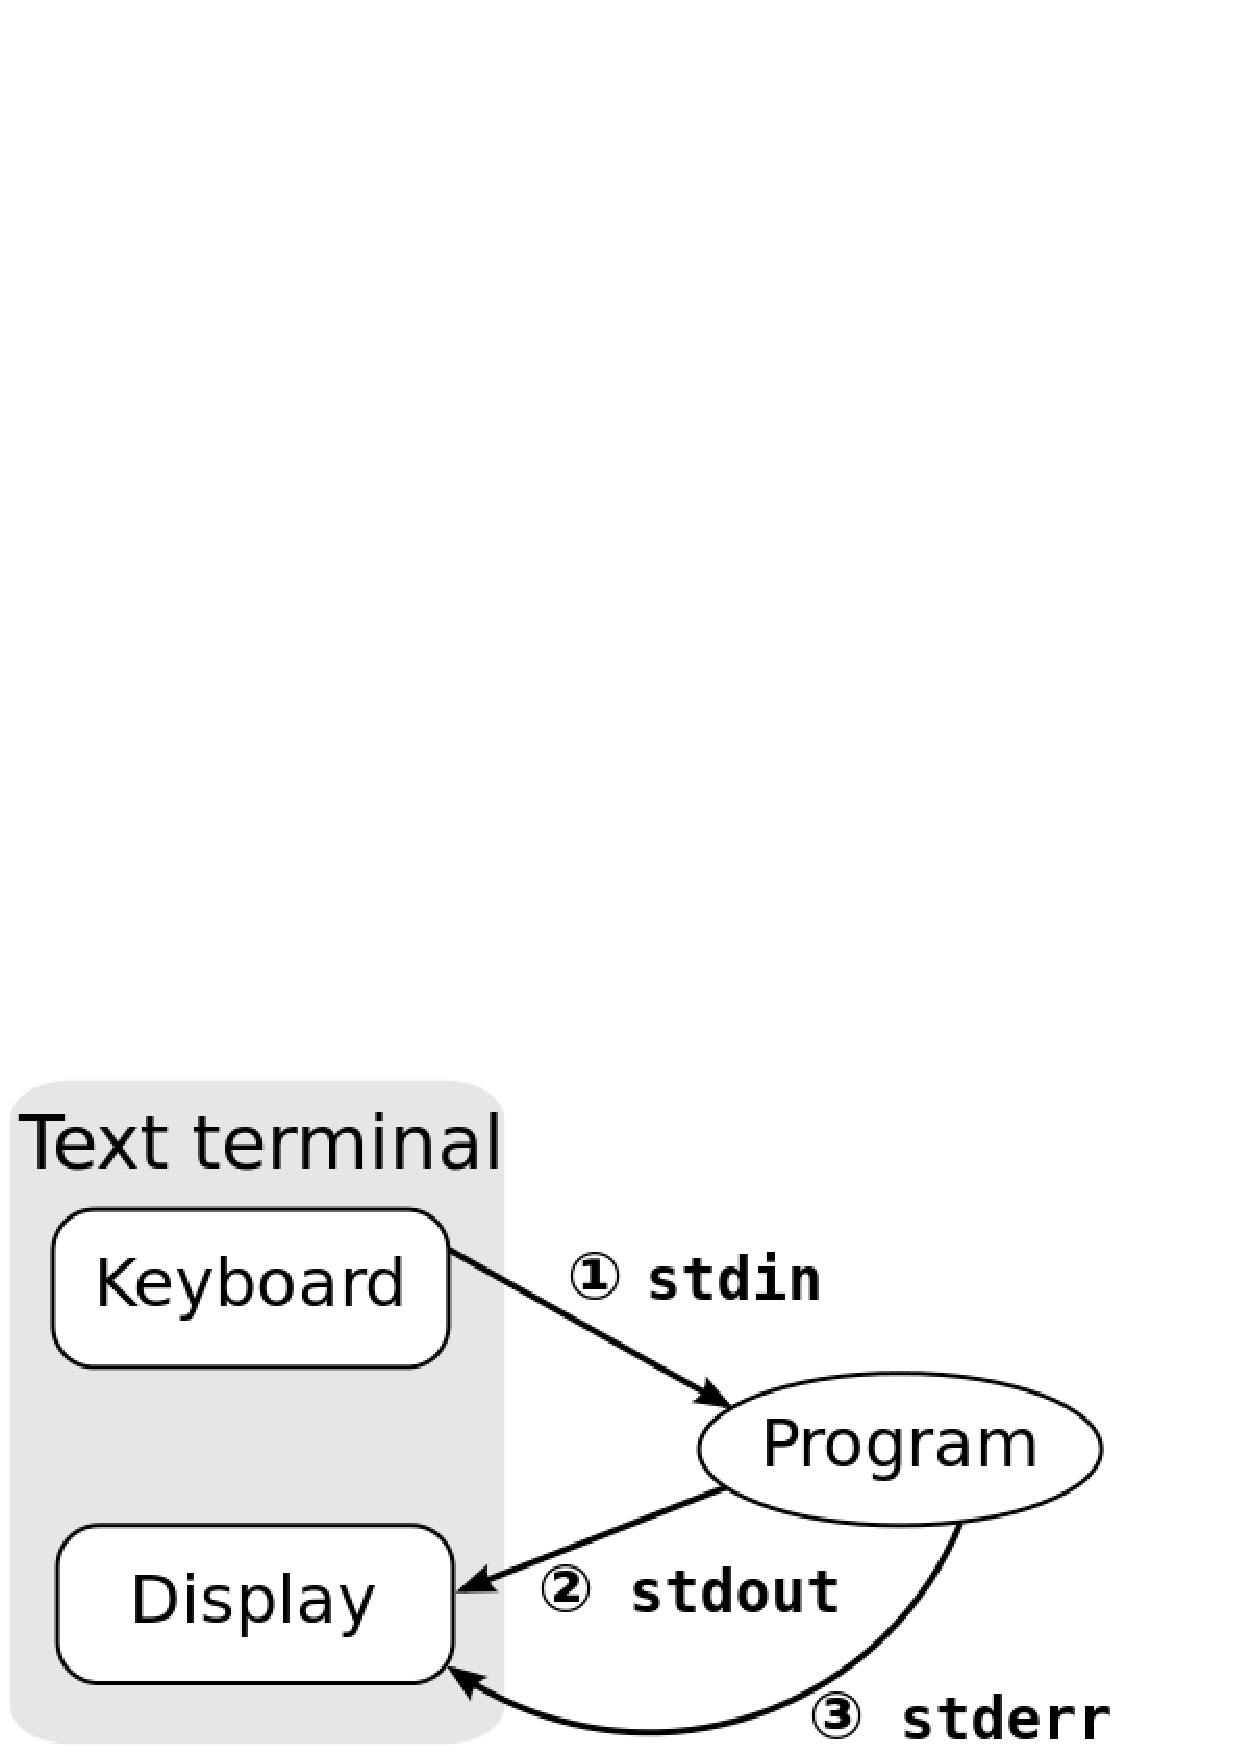
\includegraphics[width=0.5\columnwidth]{Figs/Stdstreams.png}
\caption{\label{fig:Stdstreams}Entrée standard, sortie standard et sortie d'erreur}
\end{figure}

Le terminal dans lequel vous saisissez du texte est un programme qui lit les informations saisies au clavier et les affiche. On va voir juste après qu'il est possible de chaîner des programmes de telle sorte que la sortie standard d'un programme serve d'entrée standard à un autre et ainsi construire un ``pipeline'' de traitement. 

\paragraph{Enchaîner des scripts bash: filtres et ``pipe''}

La philosophie des outils GNU consiste à écrire des outils très spécifiques et à les combiner. La combinaison de ces outils se fait par le caractère ``|'' (le pipe). La structure générale d'un pipeline est de connecter une source à un puits en appliquant successivement plusieurs filtres. Comme on va le voir, ces filtres peuvent être des commandes Bash mais rien ne vous empêche d'en écrire dans d'autres langages (comme Python). On a dit précédemment qu'une commande pouvait écrire dans sa sortie standard. En connectant deux commandes par le pipe, par exemple commande1 | commande2, la sortie standard de commande1 est connectée sur l'entrée standard de commande2. commande2 peut alors travailler sur les informations envoyées par commande1. On peut donc combiner plusieurs commandes très spécifiques pour construire un programme plus intéressant que les commandes individuelles. Par exemple, la commande \du permet de calculer l'espace occupé par des fichiers, la commande \sort permet de trier les lignes d'un fichier, on peut alors facilement lister les fichiers/répertoires du répertoire courant par ordre croissant de taille~:
\begin{center}
du * | sort -n
\end{center}

Si on ne veut afficher que les 10 plus gros fichiers/répertoires, il suffit d'afficher les 10 dernières éléments~:
\begin{center}
du * | sort -n | tail -10 
\end{center}

Si on veut compter le nombre de fichiers présents dans un répertoire~:

\begin{center}
ls -p | grep -v / | wc -l
\end{center}

Je vous laisse le soin de regarder les pages de manuel des commandes ``ls'', ``grep'' et ``wc'' pour comprendre ce qui se passe.


\subsection{Ecrire un script lisant l'entrée standard}

Pour lire depuis l'entrée standard (et on le fera souvent par la suite durant le TP), on utilisera la commande \readcmd. 

\cprotect\encadreUtilisation{
\begin{verbatim}
#!/bin/bash
while read -r ligne
do
    echo "Ligne lue : $ligne"
done
\end{verbatim}
}

Sauvegardez le script ci-dessous dans un fichier \bash{read\_input.sh} et testez le ~:
\begin{exempleResultat}
bash:\$ cat read_input.sh | ./read\_input.sh
\end{exempleResultat}

\begin{center}

\end{center}

\subsection{Avoir des informations sur l'utilisation d'une commande}

Sous linux, on peut facilement accéder à une page de manuel d'une commande à l'aide de la commande \man exécutée depuis un terminal. Par exemple, pour avoir plus d'informations sur l'utilisation de la commande \mkdir permettant de créer des répertoires, on utilisera~:

\begin{exempleResultat}
bash:\$ man mkdir
\end{exempleResultat}
On navigue alors dans le texte qui s'affiche à l'aide des flêches directionnelles. Pour quitter la page de manuelle, il suffit de presser la touche q. 

%Voir les commandes : tee et 

\vfill 
\newpage


\pagebreak

\section{TP: Revivons les grands frissons d'une éruption solaire}

Les principales éruptions solaires sont listées sur la page \url{http://en.wikipedia.org/wiki/Solar_cycle_24}.

\subsection{Introduction}

Le but de ce TP est de construire une vidéo à partir de données collectées sur le soleil par le \emph{Solar Dynamics Observatory}\footnote{http://aia.lmsal.com/index.htm}. On utilisera uniquement les images du soleil capturées à intervalle régulier. Les images sont disponibles à l'adresse \url{http://jsoc.stanford.edu/data/aia/images/}. Elles sont classées par date de mesure, la structure du répertoire distant étant~:
\begin{center}
http://jsoc.stanford.edu/data/aia/images/YYYY/MM/DD/$\lambda$/fichier.jp2
\end{center}

Le SDO observe le soleil dans différentes longueurs d'onde $\lambda \in [\mathlist{94\si{\AA}, 131\si{\AA}, 171 \si{\AA}, 193\si{\AA}, 211\si{\AA}, 304\si{\AA}, 335\si{\AA}, 1600\si{\AA}, 1700\si{\AA}, 4500\si{\AA}}]$. Pour avoir une idée des mesures à ces différentes longueurs d'onde, vous pouvez vous rendre à l'adresse \url{http://sdo.gsfc.nasa.gov/data/}, ou bien regarder l'image ci-dessous. On trouvera une description de ce qui est observé à ces différentes longueurs d'onde sur le site de la Nasa \url{http://www.nasa.gov/mission_pages/sunearth/news/light-wavelengths.html}.
\begin{figure}[htbp]
\includegraphics[width=0.65\linewidth]{Figs/solar_wavelength2.jpg}
\end{figure}

Durant ce TP, je vous propose d'utiliser les mesures à $211 \si{\AA}$. Les images sont au format JPEG2000 avec l'extension $jp2$ et une résolution de $4096 \times 4096$. Dans ce TP, on cherche à illustrer la construction de programmes du type ``puits | commande1 | commande2 ....''. On va récupérer les images, les convertir en JPEG, les redimensionner, y incruster la date et l'heure de la mesure et les combiner pour construire une vidéo. On va voir dans ce TP l'utilisation d'un certain nombre de programmes tels que \bashcmd, \wget, \convert (imagemagick), \gawk, \sed et \ffmpeg. On cherche ainsi à ne pas réinventer la roue, votre problème est de produire une vidéo à partir des images brutes et on va voir qu'en assemblant plusieurs briques déjà existantes, on peut facilement résoudre ce problème.

\begin{center}
\colorbox{lblue}{\begin{minipage}{\linewidth}
\includegraphics[width=0.05\columnwidth]{Figs/warning.png}\includegraphics[width=0.05\columnwidth]{Figs/warning.png}
\textbf{Attention}: Dans tout ce qui suit, on remplacera le préfixe des adresses web http://jsoc.stanford.edu/ par http://infomob/fix/. Sur http://infomob.metz.supelec.fr/fix/ on retrouvera plusieurs jeux d'images que j'ai récupéré de leurs serveurs, à savoir~:
\begin{itemize}
\item le 07/06/2011 en $304\si{\AA}$ : grosse éruption entre 6h et 7h
\item le 31/08/2012 en $211\si{\AA}$ et $171\si{\AA}$ : petite éruption autour de 19:00
\end{itemize}
Il y a plusieurs raisons à l'utilisation de ce miroir local: 1) les temps d'accès, 2) je crains que si tout le monde accède de manière répétée au site jsoc.stanford.edu, nous soyons banis de leur serveur web et donc qu'on ne puisse pas faire correctement le TP, 3) on ne surcharge pas inutilement leurs serveurs pour nos TPs.
\end{minipage}}
\end{center}


\subsection{Structure du projet}

Je vous propose de créer quelques répertoires pour structurer votre projet. Pour les créer, forcez vous à utiliser les commandes \mkdir, \ls, etc.. depuis un terminal.
\begin{itemize}
\item scripts : contiendra la plupart des scripts que vous écrirez,
\item raw\_images : contiendra de manière temporaire les images brutes au format .jp2,
\item images: contiendra les images converties au format jpeg et redimensionnées,
\item postproc\_images: contiendra les images jpeg dans lesquelles la date et l'heure auront été incrustées
\item video : contiendra les vidéos générées
\end{itemize}

La figure \ref{fig:soleil_overview} donne une vision d'ensemble du programme que nous allons écrire.

\begin{center}
\begin{figure}
\begin{tikzpicture}[
  font=\sffamily,
  every matrix/.style={ampersand replacement=\&,column sep=2cm,row sep=2cm},
  source/.style={draw,thick,rounded corners,fill=blue!20,inner sep=.3cm},
  datastore/.style={draw,very thick,shape=datastore,inner sep=.3cm},
  command/.style={draw,dashed, rounded corners,fill=yellow!30,inner sep=.3cm},
  dots/.style={gray,scale=2},
  to/.style={->,>=stealth',shorten >=1pt,semithick,font=\sffamily\footnotesize},
  todash/.style={->,>=stealth',shorten >=1pt,dashed,semithick,font=\sffamily\footnotesize},
  every node/.style={align=center}]

  % Position the nodes using a matrix layout
  \matrix{
    \node[source] (commande) {31/08/2012, $211 \si{\AA}$};
      \& \node[datastore] (getindex) {get\_index.sh}; 
      \& \node[command] {lynx, more, (mktemp)};\\

    \& \node[datastore] (extract) {extract\_url.sh}; 
      \& \node[command] {gawk};\\

     \& \node[datastore] (telecharge) {telecharge\_img.sh}; 
      \& \node[command] {wget};\\

     \& \node[datastore] (convert) {convert\_img.sh}; 
      \& \node[command] {convert, rm};\\

     \& \node[datastore] (date) {ecrit\_date.sh}; 
      \& \node[command] {sed, convert};\\

     \node[source] (resultat) {31\_08\_2012\_211.mp4};
     \& \node[datastore] (video) {creer\_video.sh}; 
      \& \node[command] {ffmpeg};\\    
  };

  % Draw the arrows between the nodes and label them.
  \draw[to] (commande) -- (getindex);
  \draw[to] (getindex) -- node[midway,right] {contenu de \\ http://jsoc.../2012/08/31/211/} (extract);
  \draw[to] (extract) --  node[midway,right] {URL des images \\http://jscoc.stanford..../2012\_08\_31\_\_00....jp2\\............\\ http://jscoc.stanford..../2012\_08\_31\_\_23....jp2} (telecharge);
  \draw[to] (telecharge) --  node[midway,right] {Images brutes\\./raw\_images/2012\_08\_31\_\_00....jp2\\............\\./raw\_images/2012\_08\_31\_\_23....jp2} (convert);
  \draw[to] (convert) -- node[midway,right] {Images converties et redimensionnées\\./images/2012\_08\_31\_\_00....jpg\\............\\./images/2012\_08\_31\_\_23....jpg} (date);
  \draw[todash] (date) -- node[midway,right] {Images renommées, avec date et heure\\./postproc\_images/00000.jpg\\............\\./postproc\_images/02479.jpg}(video);
  \draw[to] (video) -- (resultat);
  %% \draw[to] (buffer) --
  %%     node[midway,right] {raw event data\\level 1} (monitor);
  %% \draw[to] (monitor) to[bend right=50] node[midway,above] {events}
  %%     node[midway,below] {level 1} (storage);
  %% \draw[to] (storage) to[bend right=50] node[midway,above] {events}
  %%     node[midway,below] {level 1} (monitor);
  %% \draw[to] (monitor) -- node[midway,above] {events}
  %%     node[midway,below] {level 1} (datastore);
\end{tikzpicture}
\caption{Vue d'ensemble du TP ``Revivons les grands frissons d'une éruption solaire''.\label{fig:soleil_overview}}
\end{figure}
\end{center}

\subsection{Récupération des données d'une journée}

Le but de cette partie est d'écrire un script Bash qui se charge de récupérer les images d'une journée. Ce script prendra 4 arguments, à savoir l'année YYYY, le mois MM, le jour DD et la longueur d'onde $\lambda$ des mesures. Il devra produire en sortie le flux des URLs des images de cette journée particulière à la longueur d'onde $\lambda$.\\

Si vous allez sur le site \urlsoleil, et regardez les images du \datesoleil, vous constaterez qu'il y a énormément d'images, prises à des heures régulières mais dont on ne peut pas facilement prédire le nom de fichier. On va donc procéder différemment: on va lister l'ensemble des images disponibles dans le répertoire du \datesoleil à \lambdasoleil. Pour cela, on va utiliser l'explorateur \lynx (n'hésitez pas à appeler man lynx pour en savoir plus). \lynx est un explorateur internet textuel, sans fenêtre graphique, qui s'affiche dans la console.\\

\textbf{Lancez} \lynx et décortiquez l'interface pour effectuer une recherche de votre choix sur google.\\

Je suis d'accord avec vous, cette manière d'explorer internet n'est pas très confortable. Mais, on peut utiliser \lynx pour récupérer le contenu d'une page grâce à l'option dump 'lynx -dump URL'. En ajoutant l'option '-listonly', on ne récupère que la liste des références (les liens vers les images dans notre cas). Essayez la commande ci-dessous:
\begin{center}
\bash{lynx -dump -listonly http://jsoc.stanford.edu/data/aia/images/2012/08/31/211/ | less }
\end{center}
Il apparaît le contenu de la page, converti en texte, dans lequel vous pouvez naviguer avec les flèches directionnelles. Le contenu affiché devrait ressembler à ça~:
\begin{exempleResultat}
Références

   1. http://jsoc.stanford.edu/data/aia/images/2012/08/31/211/?C=N;O=D
   2. http://jsoc.stanford.edu/data/aia/images/2012/08/31/211/?C=M;O=A
   3. http://jsoc.stanford.edu/data/aia/images/2012/08/31/211/?C=S;O=A
   4. http://jsoc.stanford.edu/data/aia/images/2012/08/31/211/?C=D;O=A
   5. http://jsoc.stanford.edu/data/aia/images/2013/05/01/
   6. http://jsoc.stanford.edu/data/aia/images/2012/08/31/211/2012\_08\_31\_\_00\_00\_23\_34.jp2
   7. http://jsoc.stanford.edu/data/aia/images/2012/08/31/211/2012\_08\_31\_\_00\_00\_59\_34.jp2
   8. http://jsoc.stanford.edu/data/aia/images/2012/08/31/211/2012\_08\_31\_\_00\_01\_35\_34.jp2
   9. http://jsoc.stanford.edu/data/aia/images/2012/08/31/211/2012\_08\_31\_\_00\_02\_11\_34.jp2
  10. http://jsoc.stanford.edu/data/aia/images/2012/08/31/211/2012\_08\_31\_\_00\_02\_47\_34.jp2
  11. http://jsoc.stanford.edu/data/aia/images/2012/08/31/211/2012\_08\_31\_\_00\_03\_23\_34.jp2
  12. http://jsoc.stanford.edu/data/aia/images/2012/08/31/211/2012\_08\_31\_\_00\_03\_59\_34.jp2
  13. http://jsoc.stanford.edu/data/aia/images/2012/08/31/211/2012\_08\_31\_\_00\_04\_35\_34.jp2
 \end{exempleResultat}

Notez qu'on a redirigé la sortie standard de \lynx dans l'entrée standard de \less. \less est un programme qui permet de parcourir du contenu texte (e.g. un fichier mais il peut également lire depuis l'entrée standard).\\


\textbf{Écrivez} un script bash $scripts/get\_index.sh$ qui~:
\begin{itemize}
\item prenne le jour, le mois, l'année et la longueur d'onde des mesures à récupérer
\item récupère le contenu de la page grâce à lynx -dump -listonly 
%\item redirige dans la sortie standard le contenu téléchargé (on pourra utiliser le programme \cat pour afficher dans la sortie standard le contenu d'un fichier)
\end{itemize}

\subsection{Extraire les URLs des images}

Le contenu affiché par le script précédent contient beaucoup d'informations. On souhaite en extraire les URLs vers les images listées sur la page. Les URLs que nous cherchons à extraire ont un format très particulier; elles commencent par "http://"  et finissent par ".jp2". Pour filtrer les lignes qui ne contiennent que ce motif, on va utiliser \gawk et ce qu'on appelle des expressions régulières.\\

\awk est un programme qui applique un programme sur un fichier (ou l'entrée standard) ligne par ligne. Un programme awk est de la forme 'pattern \{ action \}'. \awk comprends ce mini-programme comme ``si la ligne est filtrée par le patron \emph{pattern} alors on réalise l'action \emph{action}'. Par ailleurs, \awk divise la ligne selon un séparateur (modifiable par l'option '-FS ``sep'''), qui est l'espace ' ' par défaut.\\

Prenons un exemple concret. Exécutez votre script get\_index.sh et redirigez la sortie standard dans un fichier~:
\begin{exempleResultat}
bash:\$ ./scripts/get\_index.sh 31 08 2012 211 > 31\_08\_2012\_211
bash:\$ less 31\_08\_2012\_211
\end{exempleResultat}
 
On y retrouve bien la liste des liens vers les images du \datesoleil. On va maintenant lire le fichier avec \cat et le faire passer par \awk.
\begin{exempleResultat}
bash:\$ cat 31\_08\_2012\_211 | awk '\{ print \$0 \}'
bash:\$ cat 31\_08\_2012\_211 | awk '\{ print \$1 \}'
bash:\$ cat 31\_08\_2012\_211 | awk '\{ print \$2 \}'
\end{exempleResultat}

Si vous voulez voir plus en détails la sortie de awk, n'hésitez pas à rediriger sa sortie dans less en ajoutant '| less'. Les \emph{pattern} et \emph{action} de programme \awk peuvent prendre plusieurs formes (voir \url{http://www.gnu.org/software/gawk/manual/gawk.html#Patterns-and-Actions}), on ne va en voir ici que certaines d'entre elles.  Dans l'exemple ci-dessus, nous n'avons pas précisé de \emph{pattern}, toutes les lignes sont ainsi retenues et vous avez dû constaté que la première commande affiche toute la ligne, la deuxième seulement le numéro du lien et la dernière l'adresse. Quand \awk parcours une ligne, il crée plusieurs variables utilisables dans les \emph{pattern} et \emph{action}, en particulier les variables \$0, \$1, ... \$NF qui permettent d'accéder aux champs extraits par \awk (\url{http://www.gnu.org/software/gawk/manual/gawk.html#Fields}). \$0 est une variable particulière qui contient toute la ligne lue par \awk. Les champs sont accessibles par les variables \$1, \$2, ... ; Il y a également d'autres variables, comme NF égal au nombre de champs dans la ligne, de telle sorte que \$NF sera toujours le dernier champ extrait. La variable NR contient le numéro de ligne lu, ... \\

A titre d'exemple, on peut facilement décoder la lettre envoyée par George Sand à Alfred de Musset ci-dessous~:
\begin{center}
\begin{verbatim}
Cher ami,
Je suis toute émue de vous dire que j'ai
bien compris l'autre jour que vous aviez
toujours une envie folle de me faire
danser. Je garde le souvenir de votre
baiser et je voudrais bien que ce soit
une preuve que je puisse être aimée
par vous. Je suis prête à montrer mon
affection toute désintéressée et sans cal-
cul, et si vous voulez me voir ainsi
vous dévoiler, sans artifice, mon âme
toute nue, daignez me faire visite,
nous causerons et en amis franchement
je vous prouverai que je suis la femme
sincère, capable de vous offrir l'affection
la plus profonde, comme la plus étroite
amitié, en un mot : la meilleure épouse
dont vous puissiez rêver. Puisque votre>
âme est libre, pensez que l'abandon ou je
vis est bien long, bien dur et souvent bien>
insupportable. Mon chagrin est trop
gros. Accourrez bien vite et venez me le
faire oublier. À vous je veux me sou-
mettre entièrement.
Votre poupée 
\end{verbatim}
\end{center}

en utilisant la commande awk : \bash{awk 'NR \% 2 == 1 \{ print \$0 \}'} qui permet d'afficher toutes les lignes d'indice impair. La réponse de Musset ci-dessous~:

\begin{center}
\begin{verbatim}
Quand je mets à vos pieds un éternel hommage,
Voulez-vous qu'un instant je change de visage ?
Vous avez capturé les sentiments d'un coeur
Que pour vous adorer forma le créateur.
Je vous chéris, amour, et ma plume en délire
Couche sur le papier ce que je n'ose dire.
Avec soin de mes vers lisez les premiers mots,
Vous saurez quel remède apporter à mes maux. 
\end{verbatim}
\end{center}

se décrypte facilement en utilisant awk. Le programme decode\_musset.awk ci-dessous permet en effet de le décrypter \bash{awk -f decode\_musset.awk musset\_sand.txt}. Dans le programme AWK, ORS signifie ``Output Record Separator'' c'est à dire le caractère utilisé entre chaque résultat filtré.

\begin{verbatim}
BEGIN { ORS = " " } 
{ print $1 }
END { print "? \n" }
\end{verbatim}

Le premier exemple utilise une expression arithmétique (\bash{NR \% 2 == 1}) comme \emph{pattern}. On peut également utiliser des expressions régulières. Par exemple, pour vérifier si une ligne contient une URL vers une image au format jp2, on peut utiliser la commande awk~: \bash{awk '/http:\textbackslash{}/\textbackslash{}/.*\textbackslash{}.jp2/ \{ print \$2 \}'}. Cette commande un peu étrange recherche, dans la ligne courante, une chaîne de caractère de la forme http:// (\bash{http:\textbackslash{}/\textbackslash{}/}), suivi d'un nombre arbitraire de caractères (\bash{.*}), suivi de .jp2 (\bash{\textbackslash{}.jp2}). Si cette expression régulière est vérifiée, alors le deuxième champs \$2 est affiché. \textbf{Ecrivez un script} bash \bash{scripts/extract\_url.sh} qui, étant donné la liste des références obtenues avec Lynx, produise un flux dans la sortie standard des URL des images.\\

\textbf{Testez le script} que vous venez d'écrire en lui donnant en entrée un contenu récupéré par Lynx. Je vous propose d'utiliser le fichier 2012\_08\_31\_211 que avez créé précédemment. Pour lire ce fichier et le rediriger vers l'entrée standard, nous utilisons la commande \bash{cat}. Vous pouvez donc vérifier le fonctionnement de votre script par la commande ci-dessous~:
\begin{center}
\bash{cat 31\_08\_2012\_211 | ./scripts/extract\_url.sh}
\end{center}
Cela devrait vous afficher les URLs de toutes les images. Pour n'en afficher qu'une partie, par exemple les 10 premières ou 10 dernières, vous pouvez utiliser les commandes \bash{head} et \bash{tail}~:
\begin{center}
\bash{cat 31\_08\_2012\_211 | ./scripts/extract\_url.sh | head -10}
\end{center}
Ce qui devrait produire~:
\begin{exempleResultat}
http://jsoc.stanford.edu/data/aia/images/2012/08/31/211/2012_08_31__00_00_11_63__SDO_AIA_AIA_211.jp2
http://jsoc.stanford.edu/data/aia/images/2012/08/31/211/2012_08_31__00_00_47_62__SDO_AIA_AIA_211.jp2
http://jsoc.stanford.edu/data/aia/images/2012/08/31/211/2012_08_31__00_01_23_62__SDO_AIA_AIA_211.jp2
http://jsoc.stanford.edu/data/aia/images/2012/08/31/211/2012_08_31__00_01_59_62__SDO_AIA_AIA_211.jp2
http://jsoc.stanford.edu/data/aia/images/2012/08/31/211/2012_08_31__00_02_35_62__SDO_AIA_AIA_211.jp2
http://jsoc.stanford.edu/data/aia/images/2012/08/31/211/2012_08_31__00_03_11_62__SDO_AIA_AIA_211.jp2
http://jsoc.stanford.edu/data/aia/images/2012/08/31/211/2012_08_31__00_03_47_62__SDO_AIA_AIA_211.jp2
http://jsoc.stanford.edu/data/aia/images/2012/08/31/211/2012_08_31__00_04_23_63__SDO_AIA_AIA_211.jp2
http://jsoc.stanford.edu/data/aia/images/2012/08/31/211/2012_08_31__00_04_59_62__SDO_AIA_AIA_211.jp2
http://jsoc.stanford.edu/data/aia/images/2012/08/31/211/2012_08_31__00_05_35_62__SDO_AIA_AIA_211.jp2
\end{exempleResultat}

\begin{center}
\bash{cat 31\_08\_2012\_211 | ./scripts/extract\_url.sh | tail -10}
\end{center}
ce qui devrait produire~:
\begin{exempleResultat}
http://jsoc.stanford.edu/data/aia/images/2012/08/31/211/2012_08_31__23_54_11_62__SDO_AIA_AIA_211.jp2
http://jsoc.stanford.edu/data/aia/images/2012/08/31/211/2012_08_31__23_54_47_62__SDO_AIA_AIA_211.jp2
http://jsoc.stanford.edu/data/aia/images/2012/08/31/211/2012_08_31__23_55_23_62__SDO_AIA_AIA_211.jp2
http://jsoc.stanford.edu/data/aia/images/2012/08/31/211/2012_08_31__23_55_59_62__SDO_AIA_AIA_211.jp2
http://jsoc.stanford.edu/data/aia/images/2012/08/31/211/2012_08_31__23_56_35_63__SDO_AIA_AIA_211.jp2
http://jsoc.stanford.edu/data/aia/images/2012/08/31/211/2012_08_31__23_57_11_62__SDO_AIA_AIA_211.jp2
http://jsoc.stanford.edu/data/aia/images/2012/08/31/211/2012_08_31__23_57_47_62__SDO_AIA_AIA_211.jp2
http://jsoc.stanford.edu/data/aia/images/2012/08/31/211/2012_08_31__23_58_23_62__SDO_AIA_AIA_211.jp2
http://jsoc.stanford.edu/data/aia/images/2012/08/31/211/2012_08_31__23_58_59_62__SDO_AIA_AIA_211.jp2
http://jsoc.stanford.edu/data/aia/images/2012/08/31/211/2012_08_31__23_59_35_62__SDO_AIA_AIA_211.jp2
\end{exempleResultat}

Si vous voulez savoir combien d'images sont ainsi disponibles, on peut utiliser un compteur, incrémenté chaque fois que l'expression régulière est vérifiée~:
\begin{center}
\bash{awk \textquotesingle BEGIN \{ sum = 0 \} /http:\textbackslash{}/\textbackslash{}/.*\textbackslash{}.jp2/ \{ sum = sum + 1 \} END \{ print sum \}\textquotesingle}
\end{center}
Sur le fichier de dump utilisé précédemment, cela nous donne 2426 images.

\subsection{Affichage d'une partie du flux des URL des images}

On peut maintenant tester nos deux premiers scripts en les mettant ``bout à bout''. Ecrivez un script \bash{all.sh} qui~:
\begin{itemize}
\item prenne 4 arguments que nous noterons DD, MM, YYYY, lambda
\item extrait la liste des références de la page des images à la date DD/MM/YYYY à la longueur d'onde lambda (script \bash{script/get\_index.sh})
\item et filtre son contenu pour n'afficher que les URL des images (script \bash{scripts/extract\_url.sh})
\item les affiche
\end{itemize}

Pour l'affichage, vous pourrez vérifier que vous capturez bien les premières et dernières images en n'affichant qu'une partie du flux des URLs à l'aide des commandes \head et \tail.

\subsection{Téléchargement des images}

Nous avons généré, grâce à la commande précédente, un flux dans la sortie standard d'URL des images jp2 qui nous intéressent. Nous souhaitons maintenant télécharger ces images. Pour ce faire, nous allons utiliser la commande \bash{wget}. L'utilisation la plus simple de \bash{wget} est de l'appeler par \bash{\wget url}, par exemple~:
\begin{center}
\wget http://jsoc.stanford.edu/data/aia/images/2012/08/31/211/2012\_08\_31\_\_00\_00\_23\_34\_\_SDO\_AIA\_AIA\_211.jp2
\end{center}
télécharge l'image. Vous remarquerez que l'image téléchargée est placée dans le répertoire d'appel de la commande, le répertoire courant. On souhaite que les images téléchargées soient placées dans le répertoire raw\_images. A l'aide de la page du manuel de \wget (accessible par \bash{man wget}), et en regardant en particulier les options -nd et -P, \textbf{écrivez un script} \bash{scripts/telecharge\_img.sh} qui télécharge les images dont les URLs sont fournies sur l'entrée standard et les place dans le répertoire \bash{raw\_images}\footnote{Notez qu'on pourrait aussi changer de répertoire dans le script telecharge\_img.sh, pour se placer dans raw\_images, avant de télécharger l'image}.\\

La deuxième chose à faire est d'afficher dans la sortie standard le chemin vers l'image téléchargée. Pourquoi ? parce qu'on souhaite poursuivre les traitements en indiquant au futur script de traitement d'image sur quelle image travailler. Comment faire ? Votre script \bash{scripts/telecharge\_img.sh} attends une URL dans l'entrée standard. Ce que nous allons faire, c'est utiliser awk avec pour \emph{action} d'afficher le dernier champ (\$NF) lorsque la ligne est divisée selon le séparateur '/'. Regardons un exemple~:
\begin{exempleResultat}
bash:\$ echo "http://un.exemple/durl/monimage.jp2" | awk -F/ '{print \$NF}'
monimage.jp2
bash:\$ filename=`echo "http://un.exemple/durl/monimage.jp2" | awk -F/ '{print \$NF}'`
bash:\$ echo "./raw\_images/\$filename"
./raw\_images/monimage.jp2
\end{exempleResultat}
On retrouve ici plusieurs choses. La première est l'exécution d'une commande (entre les \emph{backquotes} `...`) et l'affectation du résultat dans la variable filename. La deuxième est la construction à la volée de la chaîne de caractères correspondant au chemin vers l'image.\\

\textbf{Ajoutez l'appel} à votre script \bash{scripts/telecharge\_img.sh} dans le script \bash{all.sh}. En exécutant votre script, vous devriez voir la sortie ci-dessous~:
\begin{exempleResultat}
bash:\$ ./all.sh 31 08 2012 211
./raw_images/2012_08_31__00_00_11_63__SDO_AIA_AIA_211.jp2
./raw_images/2012_08_31__00_00_47_62__SDO_AIA_AIA_211.jp2
./raw_images/2012_08_31__00_01_23_62__SDO_AIA_AIA_211.jp2
./raw_images/2012_08_31__00_01_59_62__SDO_AIA_AIA_211.jp2
./raw_images/2012_08_31__00_02_35_62__SDO_AIA_AIA_211.jp2
./raw_images/2012_08_31__00_03_11_62__SDO_AIA_AIA_211.jp2
\end{exempleResultat}


\subsection{Traitement des images}

Nous avons récupéré une collection d'images au format JPEG2000 ``.jp2''. On souhaite 1) les convertir en jpg, 2) les redimensionner et y incruster la date/heure de la mesure. Pour cela, on va écrire un script Bash qui va essentiellement utiliser l'outil \convert sur toutes les images dont le chemin est transmis sur l'entrée standard, ainsi que quelques outils de réécriture pour transformer le nom du fichier d'image qui contient l'heure et la date de la mesure.\\

Commençons par prendre en main \convert. Comme vous pourrez le lire p.~\pageref{sec:imagemagick}, \convert est un des outils fournis par ImageMagick, GraphicsMagick, .. et qui permet de manipuler des images: convertir d'un format à un autre en appliquant éventuellement un nombre arbitraire de filtres, redimensionner les images, y introduire du texte, y appliquer des effets \footnote{l'effet polaroid est très sympa}, combiner plusieurs images, etc... \\

Commencez par vous assurer que vous disposez d'une image au format ``.jp2'' dans le répertoire raw\_images. Appelons la "img.jp2". Utilisez \convert et l'option resize pour redimensionner l'image "img.jp2" à 10\% de sa taille d'origine et la convertir en l'image "img.jpg".  Vous savez maintenant redimensionner une image, il nous reste à appliquer cette opération sur toutes les images dont le chemin est fourni sur l'entrée standard.\\

Nous \textbf{allons} (mais lisez la suite avant de commencer) écrire un script \bash{scripts/convert\_img.sh} qui va~:
\begin{itemize}
\item lire des chemins vers des images au format jp2 depuis l'entrée standard (voir p.\pageref{p:entrees_sorties_standards})
\item construire la chaîne de caractères du chemin vers l'image au format jpg (utilisez \sed), sachant que l'image cible doit être sauvegardée dans le répertoire \bash{image}
\item convertisse et redimensionne l'image source en l'image cible à 10\% de sa taille (utilisez \convert)
\item affiche dans la sortie standard le chemin vers l'image cible 
\end{itemize}

\textbf{Indications:} Pour construire le chemin vers l'image cible, il faut plusieurs choses: extraire le nom du fichier passé dans l'entrée standard (commande \basename), remplacer l'extension jp2 par jpg (utiliser \sed), concaténer le répertoire cible avec le nom du fichier image cible. Quelques exemples de ces outils sont donnés ci-dessous~:
\begin{exempleResultat}
bash:\$ basename moncheminversune/image.jp2
image.jp2
bash:\$ echo image.jp2 | sed 's/.jp2/.jpg/'
image.jpg
bash:\$ filename=image.jpg; output_path=output/\$filename; echo \$output_path
output/image.jpg
\end{exempleResultat}
On voit ici un premier exemple d'utilisation de \sed pour faire de la substitution; c'est la signification du prefixe 's' lors de l'appel à \sed. L'argument passé à \sed se lit 's/chaine de caractère source/chaine de caratère destination/'; Ainsi 's/.jp2/.jpg/' remplace la \underline{première} occurrence de ``.jp2'' par ``.jpg''; Si jamais vous voulez remplacer toutes les occurrences d'une chaine par une autre, il vous suffit d'ajouter le suffixe g, par exemple 's/.jp2/.jpg/g'.

\subsection{Incrustation de la date et de l'heure de la mesure}

On souhaite maintenant incruster la date et l'heure de la mesure dans chacune des images comme on le montre sur la figure~\ref{fig:soleil_date}. Ce qui est pratique, c'est que la date et l'heure de la mesure se trouvent dans le nom de chaque image. Il suffit donc de transformer le nom de fichier d'une image pour obtenir la chaîne de caractères à incruster dans l'image, par exemple~:
\begin{center}
2012\_08\_31\_\_00\_00\_23\_34\_\_SDO\_AIA\_AIA\_211.jpg $\Rightarrow$ 01/05/2013 00:00
\end{center}

\begin{figure}[htbp]
\begin{tabular}{cc}
\includegraphics[width=0.3\columnwidth]{Figs/soleil_date_0.jpg}&
\includegraphics[width=0.3\columnwidth]{Figs/soleil_date_1.jpg}
\end{tabular}
\caption{\label{fig:soleil_date} Image avant et après incrustation de la date}
\end{figure}

Ce travail de réécriture peut être fait à l'aide de \sed en plusieurs étapes en passant par les réécritures suivantes~:
\begin{itemize}
\item[] 2012\_08\_31\_\_00\_00\_23\_34\_\_SDO\_AIA\_AIA\_211.jpg  (1)
\item[->] 2012\_08\_31\_\_00\_00 (2)
\item[->] 2012\_08\_31 00\_00 (3)
\item[->] 01/05/2013 00:00 (4)
\end{itemize}
Le passage de (1) à (2) peut se faire en supprimant (i.e. remplacer par une chaîne vide) un motif de la forme ``\_dd...d\_dd...d\_\_SDO\_AIA\_dd...d'' o{\`u} ``dd...d'' indique une séquence de longueur arbitraire de chiffre entre 0 et 9. Le motif pour caractériser un nombre arbitraire de chiffres entre 0 et 9 est "[0-9]*". Le passage de l'étape (2) à l'étape (3) se fait en remplaçant le motif "\_\_" par " ". Le passage de (3) à (4) peut se faire facilement en utilisant la capture de groupe. Prenons un exemple~:
\begin{exempleResultat}
bash:\$ echo 2012_08_31 | sed -r 's/([0-9]*)\_([0-9]*)\_([0-9]*)/\textbackslash{}3:\textbackslash{}2:\textbackslash{}1/'
01:05:2013
bash:\$ echo 2012_08_31 | sed -r 's/([0-9]*)\_([0-9]*)\_([0-9]*)/\textbackslash{}3\textbackslash{}/\textbackslash{}2\textbackslash{}/\textbackslash{}1/'
01/05/2013
\end{exempleResultat}
On remarquera l'utilisation de l'option "-r" qui permet d'utiliser des expressions régulières étendues (par opposition aux expressions régulières de base) et facilite l'écriture de l'expression régulière pour des groupes, c'est à dire les parties de l'expression de la forme "([0-9]*)". Si nous voulions utiliser les expressions régulières de base, nous aurions dû l'écrire "\textbackslash{}([0-9]*\textbackslash{})". \\

Nous sommes maintenant capables de constuire la chaîne de caractères à insérer sur l'image. Il reste ... à l'insérer. Pour cela, on peut utiliser \convert et son "-draw". Vous pouvez tester les commandes ci-dessous sur une image redimensionnée qu'on appellera img.jpg~:
\begin{exempleResultat}
bash:\$ convert img.jpg -fill white -draw "text 0,20 'Un super texte'" res.jpg 
bash:\$ convert img.jpg -pointsize 20 -fill white -draw "text 0,20 'Un super texte'" res.jpg 
\end{exempleResultat}

Vous pouvez maintenant intégrer les deux éléments précédents dans un script \bash{scripts/ecrit\_date.sh} qui prend des chemins d'image dans l'entrée standard, et utilise convert et sed pour incruster la date et l'heure dans l'image et sauvegarder les résultats dans le répertoire \bash{postproc\_images}.\\

Il reste une dernière chose à faire dans votre script \bash{scripts/ecrit\_date.sh}. Quand nous allons regrouper les images pour en former une vidéo, il faut que les images portent des noms de fichier qui soient des nombres consécutifs, ie 00000.jpg, 00001.jpg, ... ; On peut facilement l'ajouter dans le script Bash, en utilisant un compteur incrémenté à chaque fois qu'une image est traitée et utiliser la valeur de ce compteur pour construire le nom du fichier cible. Par exemple~:
\begin{exempleResultat}
bash:\$ count=0
bash:\$ echo {\$}count
0
bash:\$ count=`expr {\$}count + 1`
bash:\$ echo {\$}count
1
\end{exempleResultat}
Vous pouvez terminer votre script en affichant dans la sortie standard le nom du fichier généré. Sachez néanmoins que notre pipeline s'arrête là. La dernière étape qui consiste à créer une vidéo à partir des images se fait une fois que tout le pipeline précédent est terminé.\\

Ajoutez l'appel à votre script \bash{scripts/ecrit\_date.sh} dans le script \bash{all.sh}.

\subsection{Et finalement, la vidéo}

Il nous reste à voir une dernière chose: comment fabriquer une vidéo à partir d'une collection d'images? En arrivant à cette partie, vous devez déjà disposer d'un script \bash{all.sh} qui, lorsqu'il est exécuté, produit une séquence d'images numérotées successivement dans le répertoire \bash{postproc\_images}, à la bonne taille, au format jpg, et dans lesquelles la date et l'heure sont incrustées.\\

De manière générale, pour produire une vidéo à partir d'une séquence d'images numérotées successivement, il existe plusieurs outils, notamment \mencoder, \ffmpeg, \avconv. Nous allons ici utiliser \ffmpeg\footnote{on notera que avconv doit succéder à \ffmpeg mais qu'à l'heure o{\`u} ce TP est écrit, il est encore instable.}.  La façon la plus simple de générer une vidéo à partir d'une collection d'images JPEG est d'appeler la commande ci-dessous~:
\begin{center}
\bash{ffmpeg -i mesimages/\%05d.jpg mavideo.mp4}
\end{center}
J'ai ici supposé que les images étaient numérotées sur 5 chiffres, c'est ce qu'indique le format \%05d, i.e. un nombre sur 5 chiffres éventuellement précédés de 0.\\

La vidéo ainsi générée peut paraître lente. C'est dû à ce qu'on appelle le \emph{frame rate}, i.e. combien d'images sont affichées par seconde. Sachant que nous disposons d'environ 2500 images pour une journée. Si on souhaite que le film ne dure que 10 secondes, il va falloir utiliser une vitesse de lecture des images de 250 images par secondes. On peut changer la vitesse de lecture de la séquence d'images en précédant l'option "-i" par une option "-r" comme suit~:
\begin{center}
\bash{ffmpeg -r 250 -i mesimages/\%05d.jpg mavideo.mp4}
\end{center}
Enfin, si on veut garantir que les images ne soient pas compressées avant d'être ajoutées au film, on peut préciser à ffmpeg l'option "-qscale 1", ce qui donne finalement~:
\begin{center}
\bash{ffmpeg -qscale 1 -r 250 -i mesimages/\%05d.jpg mavideo.mp4}
\end{center}

Pour visualiser la vidéo, vous pouvez faire appel à \mplayer~:
\begin{center}
\bash{\mplayer mavideo.mp4}
\end{center}


\begin{center}
\colorbox{lblue}{\begin{minipage}{\linewidth}
\includegraphics[width=0.05\columnwidth]{Figs/warning.png}\includegraphics[width=0.05\columnwidth]{Figs/warning.png}\includegraphics[width=0.05\columnwidth]{Figs/warning.png}
\textbf{Super important}: N'oubliez pas de faire le ménage sur votre compte en enlevant notamment les images dans les répertoires raw\_images, images et postproc\_images, sinon on va se faire gronder pour utilisation abusive de l'espace disque.
\end{minipage}}
\end{center}

\subsection{En bonus: appliquer des fausses couleurs}

Jusqu'à maintenant, nous avons utilisé des images noir et blanc. Simplement, la vidéo est beaucoup plus sympa si nous lui appliquons des fausses couleurs. Pour appliquer des fausses couleurs, une façon de faire est de se construire un gradient de couleur qui sera indéxé par la luminance de l'image. On peut par exemple créer un gradient sous gimp, ci-dessous une image 600x30 avec un dégradé ``incandescent'' et un décalage de 35.
\begin{center}
\includegraphics[width=0.7\linewidth]{Figs/soleil_gradient.jpg}
\end{center}

L'application du gradient sur l'image noir et blanc peut alors se faire grâce à imagemagick. Imagemagick sait en effet utiliser des tables de conversion de couleur~:\url{http://www.imagemagick.org/Usage/color_mods/#color_lut}
\begin{center}
\bash{\convert src.jpg -colorspace gray gradient.jpg -clut out.jpg}
\end{center}
Ce qui nous donne~:
\begin{figure}[htbp]
\begin{tabular}{cc}
\includegraphics[width=0.3\columnwidth]{Figs/soleil_greyscale.jpg}&
\includegraphics[width=0.3\columnwidth]{Figs/soleil_false_color.jpg}
\end{tabular}
\caption{\label{fig:soleil_false_color} Image avant et après colorisation.}
\end{figure}


\subsection{Notes d'installation pour refaire le TP chez vous}

Si vous voulez refaire ce TP chez vous, vous devez installer certains paquets qui ne sont pas installés par défaut. Sous Fedora, vous devez exécuter "su -c 'yum install -y ffmpeg ImageMagick mplayer'" en ayant au préalable installé les dépots rpmfusion \url{http://rpmfusion.org/}. Sous Ubuntu, "sudo apt-get install ffmpeg imagemagick mplayer" devrait faire l'affaire.


\vfill
\newpage


\pagebreak

\section{TP: Automatisons des tâches avec Makefile, Illustration pour  \LaTeX }

On a vu et on verra des commandes à exécuter dans un terminal pour
résoudre un certain nombre de problèmes (vérifier l'orthographe d'un
texte, travailler des images, regrouper des images pour créer une
vidéo, lister/modifier un ensemble de fichiers, compiler un document
\LaTeX, compiler un programme, ...). Il peut devenir difficile de se souvenir de la syntaxe
d'une commande et la syntaxe peut même devenir compliquée quand on
souhaite enchaîner des commandes. GNU Make est un des outils qui
permet d'automatiser l'exécution de tâches. L'outil \make est installé
avec le paquet \emph{make} et en général installé par défaut avec la
distribution. L'utilisation de \make passe par la
définition de fichiers Makefile qui sont traités par la commande \make. Ces fichiers peuvent s'appeler
\emph{GNUmakefile}, \emph{makefile}, ou \emph{Makefile}. Ils
contiennent un ensemble de règles avec une forme canonique:
\begin{verbatim}
cible: dépendances
       commandes
\end{verbatim}
Une règle doit être comprise comme définissant une recette de cuisine (les
commandes) permettant de construire une cible si les dépendances ont
changées. Les dépendances sont optionnelles, on en verra un exemple un
peu plus loin. \textbf{Attention} chaque ligne de \underline{commande} doit être
précédée par une tabulation. On considère un exemple
assez standard pour illustrer quelques concepts de Make, celui de
compiler un document \LaTeX. Si on veut compiler un document \LaTeX \emph{document.tex} "à la main", il faut appeler plusieurs fois \pdflatex. Si vous n'avez aucune référence bibliographique (i.e. vous n'appelez jamais ``\textbackslash{}cite") dans votre document mais des références croisées (i.e. vous appelez au moins une fois ``\textbackslash{}ref", par exemple pour faire référence à une image ou une section), il faut lancer deux fois la commande \pdflatex: le premier appel produit un fichier de référence (document.aux), le deuxième remplace chaque référence par son label. Si vous avez des références bibliographiques, il faut lancer \pdflatex, \bibtex, et \pdflatex deux fois. Comme dans le premier cas, le premier appel à \pdflatex produit une liste des références (bibliographiques et croisées) dans le fichier document.aux. L'appel à \bibtex prend en entrée le fichier document.aux, met en forme la bibliographie et produit le fichier document.bbl. Il faut maintenant intégrer cette bibliographie à votre document; c'est ce que fait l'appel suivant à \pdflatex. Enfin, un dernier appel à \pdflatex est nécessaire pour assigner, dans le document, le texte associé à une citation (son numéro par exemple). Pour résumer, pour compiler un document \LaTeX à la main, il faut exécuter, depuis un terminal, les commandes suivantes~:
\begin{center}
\bash{pdflatex document.tex ; bibtex document
  ; pdflatex document.tex; pdflatex document.tex}
\end{center}
Vous m'accorderez que c'est un peu fastidieux. Avec \make, on peut se simplifier la vie, c'est ce que nous allons voir.\\

\subsection{Première compilation d'un fichier \LaTeX avec un Makefile}

\textbf{Commencez} par récupérer un template \LaTeX qui vous plait \underline{de la section Articles} depuis le site \url{http://www.latextemplates.com/}. Je vous demande de prendre un exemple de la section Articles pour être sûr qu'il contienne des références bibliographiques. Faites l'extraction de l'archive quelque part sur votre home. Appelons par la suite ce répertoire \emph{Document}. Renommez le fichier .tex de l'archive en \emph{document.tex}. Définissez vous un fichier intitulé Makefile (sans extension, c'est pas grave!), dans lequel vous metterez le texte ci-dessous~:\\
\cprotect\encadreUtilisation{ Fichier  \textbf{Makefile}
\begin{verbatim}
document.pdf: document.tex
              pdflatex document.tex 
              bibtex document
              pdflatex document.tex 
              pdflatex document.tex
\end{verbatim}
}
Que dit cette règle ? Elle dit que la cible document.pdf dépends de la cible document.tex. Ainsi, si vous souhaitez produire la cible document.pdf mais que document.tex n'a pas changé depuis la dernière production de document.pdf, \make vous dira simplement qu'il n'y a rien à faire, i.e. on ne perds pas de temps à recompiler le document puisque son contenu n'a pas changé! Au contraire, si document.tex a changé, \make exécutera la recette de cuisine pour générer la cible document.pdf. Pour compiler votre document, il vous suffit de taper, dans le terminal \bash{make document.pdf},  et de laisser \LaTeX mouliner. Si tout s'est bien passé, vous devriez voir un fichier \emph{document.pdf} que vous pouvez ouvrir grâce à la commande \bash{evince document.pdf}\footnote{sur certaines distributions, il existe d'autres viewers PDF, comme \okular, sous Ubuntu. L'un des avantages des viewers comme \okular ou \evince, et comparé à \acroread, c'est qu'il se met automatiquement à jour si le document PDF est regénéré.}.\\

Pour se simplifier encore un peu la vie, on peut ajouter une autre règle~:\\
\cprotect\encadreUtilisation{ Fichier  \textbf{Makefile}\\
(...)
\begin{verbatim}
pdf: document.pdf
\end{verbatim}
}
Ici, c'est une règle sans recette de cuisine, juste une dépendance. Mais pour le coup, il vous suffit de taper \bash{make pdf} pour produire le document PDF.

\subsection{Une règle pour faire le ménage}

\textbf{Listez} les éléments du répertoire et vous devriez constater que nos appels à \pdflatex et \bibtex ont produits plusieurs fichiers temporaires (des fichiers .aux, .bbl, .out, .log, ...). Il y a également des fichiers temporaires produits par \emacs que vous avez utilisé pour éditer votre fichier latex et votre Makefile: ce sont les fichiers qui se terminent avec un tilde, e.g.  "document.tex\textasciitilde".\\

Pour supprimer les fichiers temporaires, il suffit de lancer la commande~: \bash{rm document.aux document.bbl document.out document.log document.tex\textasciitilde}. \underline{\textbf{ATTENTION!!}} N'oubliez pas le tilde à la fin de document.tex sinon, ben vous supprimez votre document.... \textbf{Définissez} une règle dont la cible est \emph{clean}, qui n'a pas de dépendance, et dont la recette de cuisine supprime les fichiers temporaires. \textbf{Testez la}, ça marche ?\\

\subsection{Et voila}

Finalement, le Makefile précédent est tout ce dont nous avons besoin pour produire du PDF à partir d'un fichier \LaTeX. En résumé, si vous voulez écrire en \LaTeX, il vous faut~:
\begin{itemize}
\item un bon éditeur de texte avec correction orthographique, e.g. \emacs (qui peut d'ailleurs également éditer des fichiers bitex)
\item un viewer de document PDF, e.g. \evince ou \okular
\item un Makefile pour automatiser la compilation
\end{itemize}

En passant, vous pouvez aussi réaliser des supports de présentation avec \LaTeX grâce au paquet Beamer ou dérivés. Allez voir sur le site \url{www.latextemplates.com}, dans la section Presentations.


\subsection{Allons un peu plus loin}

La règle de compilation d'un document \LaTeX est assez générique, elle n'est pas spécifique au document document.tex mais pourrait s'appliquer à n'importe quel document latex avec l'extension .tex. Avec \make, on peut définir des règles génériques et je vous propose de chercher à l'écrire en vous renvoyant à la section \ref{sec:makefile} dans laquelle cette question est abordée dans le contexte de la compilation de programme C++. \\

Enfin, sur un autre sujet, sachez que si vous souhaitez créer des illustrations dans lesquelles faire apparaître des formules mathématiques \LaTeX, vous pouvez le faire grâce à un logiciel de dessin vectoriel, certes sobre, mais très pratique: \xfig. D'ailleurs, sachez également que les dessins \xfig sont générables "à la main", c'est à dire qu'un programme peut écrire une série de commandes de tracé directement en format ASCII et vous pourrez alors importer votre figure depuis \xfig ou l'exporter vers d'autres formats (de préférence vectoriel: svg, eps, ..).

%% \subsection{En passant, et si vous vouliez faire des figures avec des notations mathématiques ?}

%% Dans la série des programmes qui peuvent paraître austaires mais qui rendent bien service, je vous propose de regarder \xfig.

%% \begin{figure}[htbp]
%% 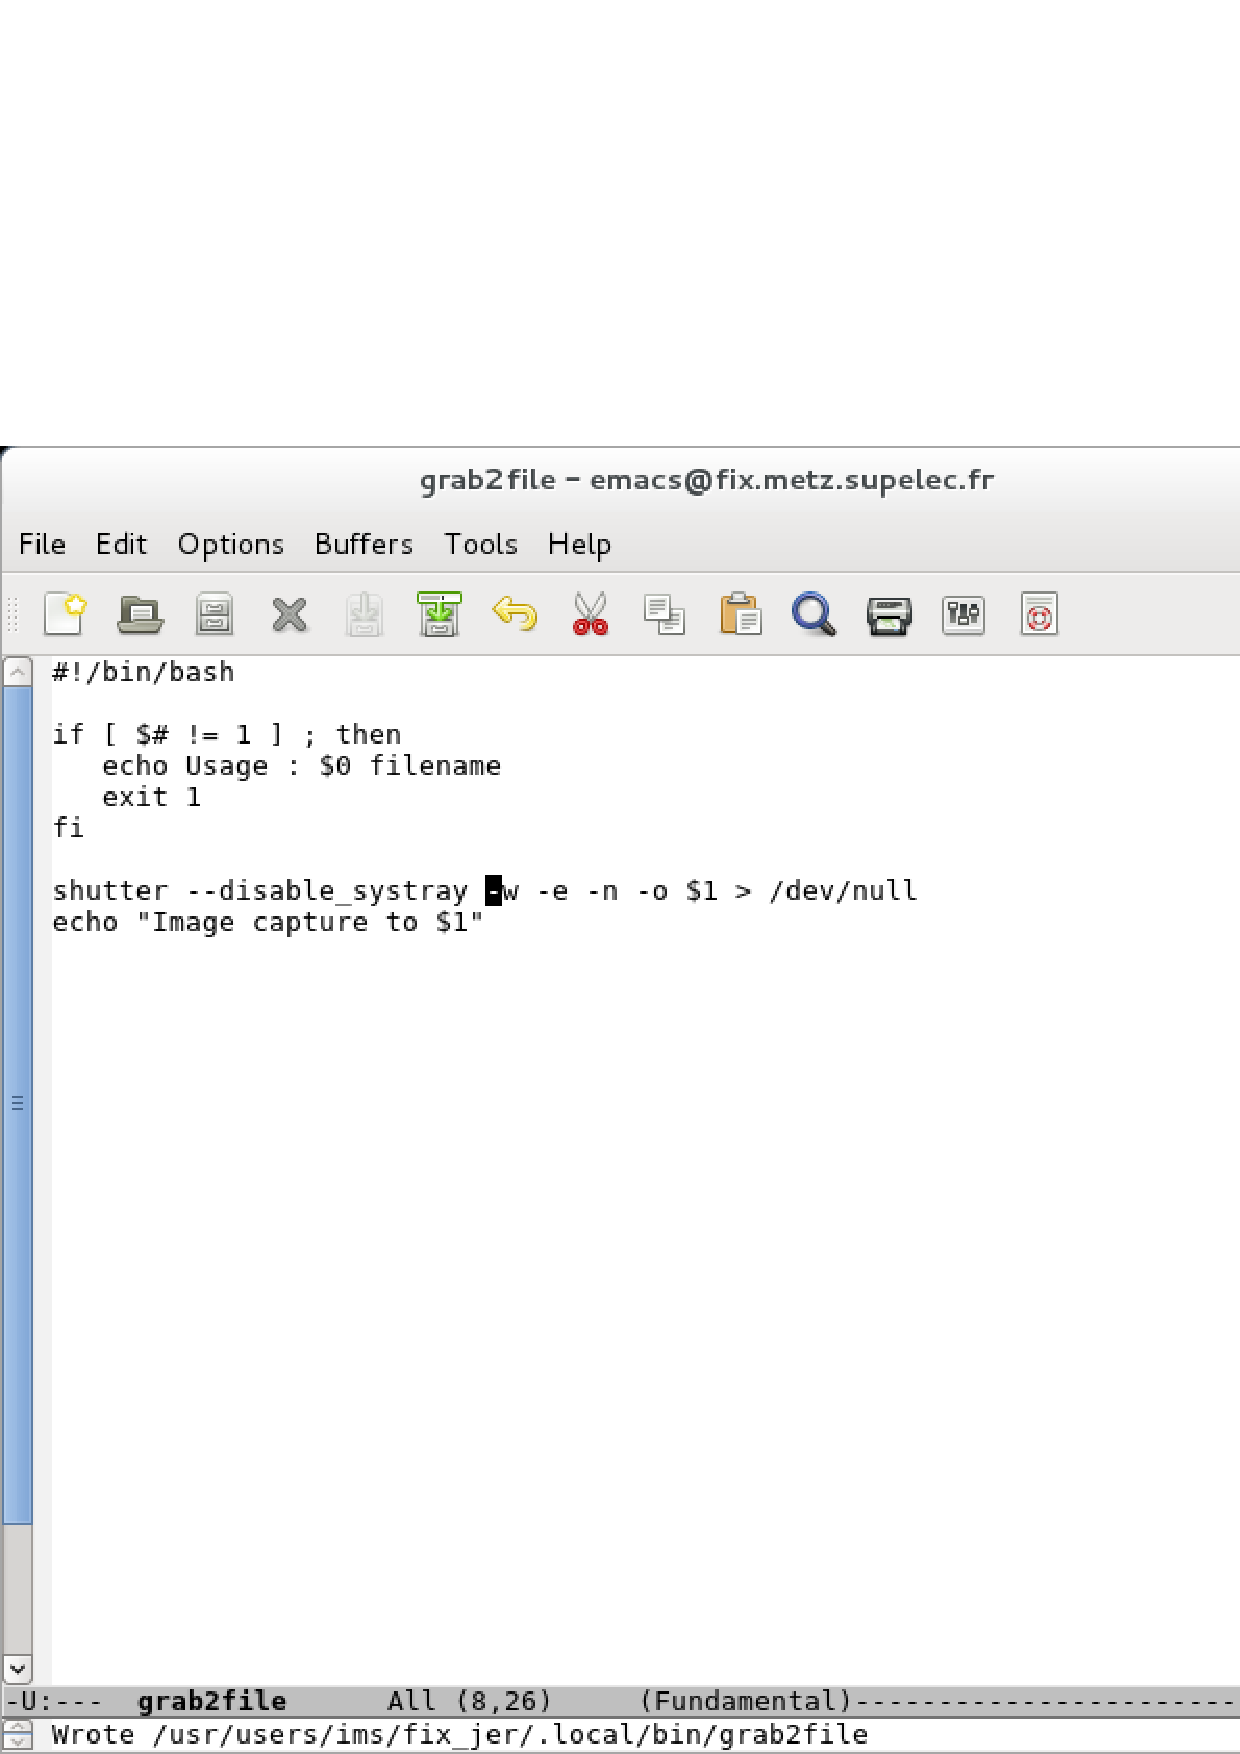
\includegraphics[width=0.5\columnwidth]{test.pdf}
%% \end{figure}


\pagebreak


\begin{figure}[htbp]
\includegraphics[width=\linewidth]{Figs/logo_meteo.png}
\end{figure}

\section{TP météo}

Cas pratique: Nous allons utiliser une base de données météo
disponible en ligne
\url{http://cdo.ncdc.noaa.gov/qclcd_ascii/}\footnote{Les informations
  qui figurent dans les fichiers sont documentées ici
  \url{http://cdo.ncdc.noaa.gov/qclcd/qclcddocumentation.pdf}}. Cette
base de données contient des archives de relevés météorologiques depuis
1996. Attention, nous utiliserons pour le moment uniquement les
données de 1996 à 2007 (le format des données a changé en 2007,
on adaptera tout à la fin du sujet notre programme pour qu'il puisse
gérer ce format légèrement différent). Nous souhaitons écrire un logiciel permettant de visualiser les évolutions de la température sur une période
donnée. Pour ce faire nous allons utiliser plusieurs des outils
disponibles sous Unix~:
\begin{itemize}
\item \zenity pour saisir les dates limites pour lesquelles effectuer le tracé,
\item \wget pour récupérer les archives de données à tracer,
\item \awk pour filtrer les enregistrements et n'extraire que les
  données à tracer,
\item \python et le module \href{http://matplotlib.org/basemap/users/examples.html}{basemap} pour tracer effectivement les données sélectionnées,
\item \imagemagick pour post-traiter les images ,
%\item \zenity pour afficher des informations sur l'avancement du
%  traitement des images
\item \ffmpeg pour générer une vidéo des images tracées
  précédemment
\item \makefile ou \bashcmd pour encapsuler l'ensemble dans un script et
  qui gérera l'exécution de tous les processus précédents
\end{itemize}

\subsection{Présentation du projet}

Les données météo que nous allons utiliser sont disponibles en ligne
\url{http://cdo.ncdc.noaa.gov/qclcd_ascii/} et fournies par le
National Climatic Center de la National Oceanic and Atmospheric
Administration (NOAA). Les archives nommées AAAAMM.tar.gz
contiennent les mesures pour le mois MM de l'année AAAA. Les archives de ces données (les .tar.gz)
contiennent 5 fichiers. 
\begin{itemize}
\item station.txt : description des stations d'enregistrements
  (identifiant WBAN, latitude, longitude, etc..)
\item AAAAMMhpd.txt : mesure des précipitations
\item AAAAMMhourly.txt, AAAAMMdailyavg.txt, AAAAMMdaily.txt : mesures
  heure par heure ou journalières\\
\end{itemize}

Nous utiliserons par la suite uniquement les fichiers \textbf{station.txt} et
\textbf{AAAAMMdaily.txt}. Les fichiers de mesures contiennent les mesures de
température, force du vent etc.. et sont indexées par l'identifiant
WBAN (\emph{Weather-Bureau-Army-Navy}) de la station de mesure. Pour tracer la carte des températures en
une date donnée, il faudra donc~:
\begin{itemize}
\item récupérer l'archive mensuelle qui contient les mesures de cette date
\item filtrer le fichier de mesure AAAAMMdaily.txt pour en extraire
  les mesures à la date souhaitée
\item combiner ces mesures avec le fichier station.txt pour formater
  les données à fournir au script de tracé (voir plus bas)
\item tracer ces données
\end{itemize}

\begin{center}
\begin{figure}
\begin{tikzpicture}[
  font=\sffamily,
  every matrix/.style={ampersand replacement=\&,column sep=2cm,row sep=2cm},
  source/.style={draw,thick,rounded corners,fill=blue!20,inner sep=.3cm},
  datastore/.style={draw,very thick,shape=datastore,inner sep=.3cm},
  command/.style={draw,dashed, rounded corners,fill=yellow!30,inner sep=.3cm},
  dots/.style={gray,scale=2},
  to/.style={->,>=stealth',shorten >=1pt,semithick,font=\sffamily\footnotesize},
  todash/.style={->,>=stealth',shorten >=1pt,dashed,semithick,font=\sffamily\footnotesize},
  every node/.style={align=center}]

  % Position the nodes using a matrix layout
  \matrix{
    \node[source] (commande) {Requête 01/06/2007 -> 15/07/2007};
      \& \node[datastore] (date) {Generate dates}; 
      \& \node[command] {zenity, awk};\\

    \& \node[datastore] (getdata) {Get data}; 
      \& \node[command] {wget, tar, awk};\\ 

    \& \node[datastore] (plotdata) {Plot data}; 
      \& \node[command] {python (module basemap)};\\ 

      \node[source] (output) {01/06/2007\_15/07/2007.mp4};
    \& \node[datastore] (video) {Create video}; 
      \& \node[command] {ffmpeg};\\ 
  };

  % Draw the arrows between the nodes and label them.
  \draw[to] (commande) -- (date);
  \draw[to] (date) -- node[midway,right] {01/06/2007,\\ 02/06/2007,\\ ... ,\\ 15/07/2007} (getdata);
  \draw[to] (getdata) -- node[midway,right] {data/01062007.txt, \\ data/02062007.txt,\\ ... ,\\ data/15072007.txt\\ data/200706daily.txt, data/200706station.txt,\\ data/200707daily.txt, data/200707station.txt} (plotdata);
  \draw[todash] (plotdata) -- node[midway,right] {images/01062007.png, \\ images/02062007.png,\\ ... ,\\ images/15072007.png} (video);
 \draw[to] (video) -- (output);
\end{tikzpicture}
\caption{Vue d'ensemble du TP ``Météo''.\label{fig:meteo_overview}}
\end{figure}
\end{center}

Je vous propose la conception sur la figure \ref{fig:meteo_overview}. Prenons le temps de la comprende. Nous souhaitons que l'utilisateur puisse préciser deux dates pour indiquer la période du tracé des mesures (zenity, p.\pageref{sec:zenity}, va nous aider pour ça). Un module est alors en charge de générer la séquence des jours séparant ces deux dates limites (on utilisera un petit script awk et les commandes mktime et strftime). L'idée est ici de très tôt se coller au format du flux d'image que nous souhaitons produire en sortie (i.e. une image par jour) et de s'adapter ensuite au format des données. Ensuite, étant donnée une date, e.g. 01/06/2007, on se débrouille pour construire l'URL vers le fichier de données et le télécharger à l'aide de awk. On doit maintenant produire un fichier de données spécifique à la journée et aux données à tracer; on facilite ainsi les traitements suivants en excluant beaucoup de données inutiles et en faisant le boulot de la fusion des données géographiques sur les stations et des mesures à proprement parler. Arrivée là, on a quasiment terminé le travail. Il suffit de tracer les données météo et on utilisera Python et le module Basemap (\url{http://matplotlib.org/basemap/}) pour cela\footnote{On peut faire des tracés très sympa avec basemap!!}. On se retrouve alors avec une collection d'images qu'il nous suffit d'assembler à l'aide de \ffmpeg. 

\subsection{Mise en place du projet}

On va commencer par structurer notre répertoire de travail avec les
répertoires et fichiers ci-dessous.

\begin{center}
\tikzstyle{file}=[anchor=west]
\tikzstyle{dir}=[draw=black,thick,anchor=west]
\begin{tikzpicture}[%
  grow via three points={one child at (0.5,-0.7) and
  two children at (0.5,-0.7) and (0.5,-1.4)},
  edge from parent path={(\tikzparentnode.south) |- (\tikzchildnode.west)}]
  \node [dir] {Meteo}
    child { node [dir] {data}}
    child { node [dir] {images}}
    child { node [dir] {videos}}
    child { node [dir] {scripts}};
\end{tikzpicture}
\end{center}

\textbf{Définissez} un script bash clean.sh qui supprime tout les éléments des répertoires data, images et videos.

\subsection{Interface pour la requête - \zenity}

La première étape consiste à fournir à l'utilisateur une interface simpliste pour saisir les dates de début et de fin de la période à tracer. Comme on ne souhaite pas une interface très évoluée, on va faire appel à un outil très pratique, \zenity. Commençons par voir ce qu'on peut faire avec \zenity sachant que vous trouverez une liste complètes des éléments graphiques créables avec \zenity dans le \href{https://help.gnome.org/users/zenity/stable/}{manuel}. Ici, on s'intéresse essentiellement à créer une boite de dialogue avec deux zones de texte pour saisir nos dates, quelque chose qui ressemble à la figure \ref{fig:zenity_temperature}.\\

\myfig{Figs/zenity_temperature.png}{\label{fig:zenity_temperature}Interface Zenity pour saisir les dates de début et de fin de l'animation des températures sur le territoire Américain.}

Exécutez l'exemple ci-dessous. 
\begin{exempleResultat}
bash:\$ zenity --forms --text="Test" --add-entry="Une entrée"
bash:\$ zenity --entry --text="Test"
\end{exempleResultat}
Saisissez un texte dans la zone de texte et validez. Vous observez alors que le texte que vous avez saisi s'affiche dans le terminal; le résultat de la commande est alors le texte que vous avez entré. On a déjà vu dans les TP précédents qu'il est possible d'exécuter des commandes depuis un script bash et grâce à zenity, vous pouvez même facilement ajouter des éléments graphiques (basiques, je vous l'accorde, mais ça nous suffit ici!). A l'aide de l'aide en ligne sur \zenity, à vous de réaliser l'interface graphique dont nous avons besoin pour saisir nos deux dates. Celle de la figure \ref{fig:zenity_temperature} contient un \textbf{formulaire} avec deux \textbf{entrées} texte et un \textbf{titre} (\textbf{Attention}, sur les anciennes versions de zenity (par exemple celle avec la Fedora 14), la première solution n'existe pas. Il faudra donc faire deux appels successifs à "zenity --entry.." pour saisir respectivement les dates de début et de fin). Pour des raisons pratiques pour la suite, \underline{assurez-vous} que le \textbf{separateur} est le caractère d'espace.\\

\textbf{Placez} l'appel à zenity dans un script bash que nous appellerons get\_date.sh.


\subsection{Génération de la séquence de dates - \python}

Il nous faut maintenant, à partir de deux dates limites, produire la séquence des dates qui les sépare. Appelons ce script que nous aimerions écrire generate\_dates.sh, et voyons ce que nous aimerions que ce script fasse.
\begin{exempleResultat}
bash:\$ echo "01/06/2007 15/07/2007" | ./generate\_dates.py 
01062007
02062007
03062007
...
15072007
\end{exempleResultat}
On aimerait donc produire une séquence date. Pourquoi ? Parce qu'on va définir un pipeline qui sera en charge de produire le flux d'images 01062007.png, 02062007.png, ..., 15072007.png. Comment faire ? Comment toujours, on a plusieurs solutions. Il en existe une avec \href{http://stackoverflow.com/questions/4351282/how-to-generate-a-sequence-of-dates-given-starting-and-ending-dates-using-awk-of}{awk}, elle est courte mais pas très rigolote. Je vous propose de voir, au détour de notre problème, l'utilisation de Python (ce sera notre première application de python et une autre suivra bientôt). La solution que nous allons proposer est, je trouve, beaucoup plus intelligible que la version awk.\\

On va donc faire un peu de Python. Pour faire du python, vous pouvez soit définir un script (i.e. un fichier texte dont l'extension est habituellement ".py") soit l'utiliser directement dans le terminal. Avant d'écrire un script qui va générer la séquence des dates, je vous propose de commencer par voir un peu de syntaxe Python directement dans l'interpréteur. Lançons python~:
\begin{exempleResultat}
bash:\$ python
Python 2.7.5+ (default, Sep 19 2013, 13:49:51) 
[GCC 4.8.1] on linux2
Type "help", "copyright", "credits" or "license" for more information.
>>>
\end{exempleResultat}

Pour manipuler les dates, il existe le module Python \href{http://docs.python.org/2/library/datetime.html}{datetime}. Pour importer ce module, il suffit d'utiliser la commande import~:
\begin{exempleResultat}
>>> import datetime
\end{exempleResultat}
On peut maintenant instantier des objets du type datetime du module datetime. Par exemple, pour représenter le 01/06/2007 à l'aide d'un objet datetime, on utilisera le code ci-dessous (voir la \href{http://docs.python.org/2/library/datetime.html#datetime.datetime}{documentation})~:
\begin{exempleResultat}
>>> begin = datetime.datetime(day=1, month=6, year=2007)
>>> begin = datetime.datetime(2007, 6, 1)
>>> begin
datetime.datetime(2007, 6, 1, 0, 0)
\end{exempleResultat}
La première façon de construire un objet de type datetime utilise des arguments nommés, la seconde des arguments positionnels (voir la \href{http://docs.python.org/2/glossary.html#term-argument}{documentation}). L'un des avantages des paramètres nommés est de pouvoir les positionner dans l'ordre que l'on souhaite. Ce type datetime nous permet de manipuler des dates. Il fournit notamment des opérateurs pour incrémenter une date d'une durée (type \href{http://docs.python.org/2/library/datetime.html#datetime.timedelta}{datetime.timedelta}) arbitraire, de les convertir en une chaîne de caractères avec un format déterminé, de vérifier si une date précède une autre date, etc... Voici quelques exemples~:
\begin{exempleResultat}
>>> nextday = begin + datetime.timedelta(days=1)
>>> nextday
datetime.datetime(2007, 6, 2, 0, 0)
>>> nextday = begin + datetime.timedelta(days=3994)
>>> nextday
datetime.datetime(2018, 5, 8, 0, 0)
>>> print(nextday.strftime("%d/%m/%Y''))
08/05/2018
>>> begin < nextday
True
>>> begin > nextday
False
\end{exempleResultat}
Il nous manque encore quelques ingrédients pour pouvoir écrire notre script generate\_dates.py~:
\begin{itemize}
\item comment récupérer des arguments passés par l'entrée standard à un script python
\item les arguments récupérés étant des chaînes de caractères de la forme dd/mm/YYYY, comment y extraire les entiers correspondants au jour, mois et année
\item comment itérer entre deux dates
\end{itemize}
Pour récupérer les arguments passés à un script python, qu'on appellerai \bash{python script.py titi ttoto 12}, on utiliserait le module "sys" et son attribut, de type liste, sys.argv. Ici, nous allons procéder de manière un peu différente puisqu'on souhaite passer les arguments \underline{par l'entrée standard}, i.e. quelque chose du type~:
\begin{center}
\bash{echo "01/06/2007 15/07/2007" | ./generate\_dates.py}
\end{center}
J'ai ici utilisé echo pour avoir un exemple sous la main pour tester mais en pratique c'est votre script get\_dates.sh qui nous fournirait dans la sortie standard les dates limites. En python, on peut lire directement de stdin\footnote{on peut même itérer sur le descripteur de fichier sys.stdin, mais cette approche bufferise la lecture...}. Même si la syntaxe ci-dessous a l'air un peu compliqué, c'est à ma connaissance la seule qui garantisse que python ne bufferise pas ses entrées et les traite bien dés qu'elles sont émises par le script qui écrit dans son entrée standard. Un exemple de script python, que nous appellerons test\_stdin.py, est donné ci-dessous~:\\

\cprotect\encadreUtilisation{ Fichier  \textbf{test\_stdin.py}
\begin{verbatim}
#!/usr/bin/python

import sys

while(True):
    l = sys.stdin.readline()
    if(l == ''):
        break
    sys.stdout.write("[test_stdin.py] a lu %s " % l)

\end{verbatim}
}

Prenez vous un fichier texte, appelons le monfichier et testez le script ci-dessus~:
\begin{center}
cat monfichier | ./test\_stdin.py
\end{center}

Testons le maintenant avec le type d'entrée qu'il va recevoir~:
\begin{center}
echo "01/06/2007 15/07/2007" | ./test\_stdin.py
\end{center}

Maintenant, il va falloir travailler un peu la ligne lue puisque je vous rappelle que nous devons récupérer des entiers correspondants au jour, mois et année des dates de début et fin. Ce qu'on cherche essentiellement à faire, c'est diviser les chaînes de caractères pour 1) isoler la date de début de la date de fin 2) extraire les éléments de chacune des dates. Testez les exemples ci-dessous~:
\begin{exempleResultat}
>>> l = "01/06/2007 15/07/2007".split()
>>> print(l)
['01/06/2007', '15/07/2007']
>>> begin=l[0].split("/")
>>> print(begin)
['01', '06', '2007']
>>> dd=int(begin[0])
>>> mm=int(begin[1])
>>> yyy=int(begin[2])
\end{exempleResultat}

Vous disposez maintenant de tout les éléments pour écrire le script python generate\_dates.py. Testez le~:
\begin{exempleResultat}
bash:\$ echo "01/06/2007 15/07/2007" | ./generate\_dates.py 
01062007
02062007
03062007
...
15072007
bash:\$ ./get\_dates.sh | ./generate\_dates.py 
\end{exempleResultat}

\subsection{Téléchargement, extraction et filtrage des données - \tar \wget \grep \awk \sed}

Maintenant que nous disposons d'un générateur des dates (generate\_dates.py produit la séquence des dates dans la sortie standard), nous pouvons gérer la partie qui consiste à télécharger les données nécessaires au tracé. Nous allons écrire ce script en Bash. Vous vous rappelez que nous disposons de données journalières au sein d'une archive mensuelle. C'est à dire que pour tracer l'archive "http://cdo.ncdc.noaa.gov/qclcd\_ascii/200706.tar.gz" contient toutes les données pour tout les jours du mois de juin. Il faut donc que notre script de téléchargement/extraction fasse plusieurs choses, étant donnée une date d'entrée~:
\begin{enumerate}
\item vérifie si l'archive du mois de la date n'est pas déjà téléchargée. Si elle ne l'est pas, on la télécharge, on l'extrait dans le répertoire data (et on renomme le fichier station pour lui ajouter le préfixe YYYYMM)
\item filtre le fichier de données pour construire un fichier de données spécifique à la date qui nous intéresse.
\end{enumerate}


\paragraph{Génération des noms des archives:}
Commençons par le premier point. Ecrivez un script bash get\_data.sh qui lise l'entrée standard. Maintenant il faut extraire ce que nous lisons de l'entrée standard (e.g. 01062007) le jour, le mois et l'année. En bash, on peut extraire des sous-chaînes d'une chaîne s par l'appel "\$\{s:debut:longueur\}", par exemple~:
\begin{exempleResultat}
bash:\$ date="01062007"; echo "Day : \$\{date:0:2\}"
Day : 01
\end{exempleResultat}
Vous devriez donc maintenant pouvoir compléter votre script pour qu'il construire la chaîne de caractère correspondant à l'archive dans laquelle se trouve les données d'une journée. Par exemple, pour le 01/06/2007, cela doit donner 200706.tar.gz.\\

\paragraph{Récupération des données brutes d'une journée:}

Maintenant que nous disposons du nom de l'archive, e.g. 200706.tar.gz, on va d'abord vérifier si le fichier local Data/200706.tar.gz existe déjà, sinon on le récupère\footnote{En pratique, on pourrait être un peu plus malin. On ne va retenir qu'une partie des données de l'archive. L'archive est grosse. On pourrait donc vérifier si les données extraites et retenues de l'archive sont déjà présentes}. En bash, pour vérifier si un fichier existe, on utilise le test conditionnel "if [ -f filename ]", par exemple~:

\cprotect\encadreUtilisation{ Fichier  \textbf{file\_exists.sh}
\begin{verbatim}
#!/bin/bash

echo "Ce script teste l'existence d'un fichier passé en argument"

if [ $# != 1 ]
then
    echo "Vous devez passer un fichier en argument"
    exit
fi

if [ -f $1 ]
then
    echo "Le fichier $1 existe !"
else
    echo "Le fichier $1 n'existe pas !"
fi
\end{verbatim}
}
Vous pouvez compléter votre script get\_data.sh pour qu'il teste si l'archive recherchée est déjà disponible en local et sinon la télécharger (souvenez vous de \wget utilisé dans le premier TP).\\

\paragraph{Extraction des données pertinentes:} L'archive que nous venons de télécharger est une archive ".tar.gz". Pour l'extraire, nous utilisons l'outil \tar~:
\begin{center}
\tar   -zxf monarchive.tar.gz
\end{center}
Que signifient ces options\footnote{n'hésitez pas à aller jeter un oeil au manuel: man tar} ? "-x" signifie qu'on extrait (on pourrait aussi créer une archive avec "-c"), "-f" signifie qu'on utilise un fichier (on peut (dé-)compresser l'entrée standard :) ) et "-z" qu'on compresse avec gzip (il existe d'autres méthodes de compression).\\

On peut même faire mieux en spécifiant quels fichiers nous souhaitons extraire de l'archive. En effet, nos archives contiennent plus de fichiers que nécessaires et nous ne voulons en extraire que les fichiers xxxxdaily.txt et station.txt. Il suffit de le spécifier sur la ligne de commande~:
\begin{center}
\tar -zxf monarchive.tar.gz monfichier1.txt monfichier2.txt chemin/vers/monfichier3.txt
\end{center}

Vous savez maintenant comment extraire les deux fichiers "station.txt" et "xxxdaily.txt". On va réaliser une dernière opération sur le fichier station.txt qui consiste à en extraire uniquement les données de WBAN, latitude et longitude. A l'aide de \awk, extrayez les 3 champs pertinents et redirigez la sortie de votre appel \awk dans le fichier xxxxstation.txt avec xxxx un prefixe de la forme YYYYmm. Vous pourrez alors également supprimer le fichier station.txt et l'archive xxxx.tar.gz.

\paragraph{Filtrage des données pertinentes du fichier daily: \awk, \sed, \join}

Pour pouvoir effectuer notre tracé des températures sur le territoire américain, il nous faut plusieurs choses: les températures et les positions géographiques des enregistrements. Les fichiers xxxxdaily.txt contiennent énormément d'informations, dont un grand nombre est inutile pour notre application. Les stations d'enregistrement dans les fichiers xxxxdaily.txt sont indexées par leur WBAN mais la position géographique d'une station est quand à elle disponible dans le fichier xxxxstation.txt que nous venons de créer. Il nous faut donc extraire uniquement les températures et les WBAN du fichier xxxxdaily.txt et combiner cela avec le fichier de station. Nous allons pour cela utiliser plusieurs outils en un pipeline. Si vous inspectez un fichier xxxxdaily.txt, vous pouvez remarquer que parfois, la température est égale à M correspondant à une entrée invalide, parfois elle est suffixée par une étoile; on aimerait d'une partie supprimer les entrées invalides et d'autre part supprimer les "*" suffixant certaines températures; définissions un pipeline avec~:
\begin{enumerate}
\item \awk pour extraire uniquement les WBAN et températures moyennes de la date considérée
\item \awk pour supprimer les entrées pour lesquelles la température est égale à "M", ce qui correspond à une entrée invalide
\item \sed pour substituer les "*" par un caractère vide ""
\end{enumerate}
Enfin, utilisez \join pour combiner les données ainsi générées avec le fichier xxxxstation.txt. \join peut prendre deux fichiers en argument pour les combiner mais il accepte également qu'on remplace un des fichiers par l'entrée standard en précisant "-" comme nom de fichier; voyons quelques exemples~:
\begin{exempleResultat}
bash:\$ cat toto.txt
a a1
b b1
c c1
bash:\$ cat titi.txt
a a2 a3
b b2 b3
c c2 c3
bash:\$ join toto.txt titi.txt
a a1 a2 a3
b b1 b2 b3
c c1 c2 c3
bash:\$ cat toto.txt | join - titi.txt
a a1 a2 a3
b b1 b2 b3
c c1 c2 c3
\end{exempleResultat}
L'intérêt de la dernière commande est de pouvoir mettre l'appel \join dans un pipeline pour combiner à la volée l'entrée standard avec un fichier. Vous devriez maintenant avoir tout les éléments pour produire un fichier de données qui contiennent les WBAN, longitudes, latitudes et températures moyennes mesurées. Par exemple, vous devriez pouvoir produire le fichier 01062006.txt ci-dessous.
\begin{exempleResultat}
bash:\$ cat Data/01062006.txt
03013 38.04 -102.41 67 
03016 39.32 -107.44 64 
03017 39.50 -104.4 63 
03024 35.42 -101.23 73 
03026 39.14 -102.17 62
03027 35.00 -105.4 63 
03028 37.17 -102.37 66
....
\end{exempleResultat}

\subsection{Tracé des données - \python}

Il nous reste maintenant à effectuer le tracé des données extraites. On va partir d'un fichier de données exemple comme Data/01062006.txt. Les mesures sont ponctuelles et nous aimerions les interpoler sur tout le territoire. Nous aimerions également tracer ces données sur une carte du territoire américain. Pour cela, nous allons utiliser Python et ses modules scipy pour l'interpolation et basemap pour le tracé des cartes. Nous allons procéder par étape~:
\begin{enumerate}
\item tracer la carte
\item récupérer les données brutes et les tracer sur la carte 
\item interpoler ces données sur une grille et tracer les données interpolées
\item limiter le tracé aux terres
\end{enumerate}

\subsubsection{Tracé de la carte}
Pour tracer la carte du territoire américain, nous utilisons le module \href{http://matplotlib.org/basemap/}{basemap}. Inspirez vous du script d'exemple de basemap sur \href{http://matplotlib.org/basemap/users/cyl.html}{les projections cylindriques} pour effectuer un tracé du territoire américain. Un exemple de tracé est représenté sur la figure~\ref{fig:meteo_coastlines}.\\

\begin{figure}[htbp]
\includegraphics[width=0.7\linewidth]{Figs/meteo_coastlines.png}
\caption{\label{fig:meteo_coastlines} Tracé du territoire américain grâce au module basemap.}
\end{figure}

\subsubsection{Tracé des données brutes}
La deuxième étape consiste à importer les données précédemment filtrées et à les tracer sur la carte. Pour charger des données d'un fichier texte, organisées en colonnes, le plus simple est d'utiliser la fonction loadtxt du module \href{http://www.numpy.org/}{numpy}. Le script ci-dessous vous montre un exemple d'utilisation~:\\
\cprotect\encadreUtilisation{ Fichier  \textbf{load\_data.py}
\begin{verbatim}
#!/usr/bin/python
# -*- coding: utf-8 -*-

import sys
import numpy as np
import matplotlib.pyplot as plt

print("Ce test le chargement de données")

if(len(sys.argv) != 2):
    print("Usage : {} datefile".format(sys.argv[0]))
    sys.exit(-1)

# On récupère le chemin vers les données
datafile=sys.argv[1]

# On les charge
data = np.loadtxt(datafile)

# Et pour rigoler, on trace les températures
plt.figure()
plt.plot(data[:,3])
plt.title("Températures moyennes (deg K)")
plt.show()

\end{verbatim}
}

Ces données forment un ensemble non structuré de points; pour les tracer, nous utilisons ce qui s'appelle un \emph{scatter plot}. Mais, pour correctement tracer les données, il faut d'abord projeter les longitudes et latitudes des points de mesure sur la carte. L'object Basemap que nous avons construit lors du tracé de la carte peut être appliqué à des vecteurs de longitudes et latitudes pour calculer leur projetés.\\
\cprotect\encadreUtilisation{ Fichier  \textbf{load\_data.py}
\begin{verbatim}
...
# On suppose que data est un vecteur à 3 colonnes
# data[:,0] contient les longitudes
# data[:,1] contient les latitudes
# data[:,2] contient les températures

m = Basemap(projection='cyl',
            llcrnrlat=25,urcrnrlat=50,
            llcrnrlon=-130,urcrnrlon=-60,resolution='l')

x, y = m(data[:,0], data[:,1])
fig = plt.figure()
m.drawcoastlines()
plt.scatter(x, y, c=data[:,2])
plt.show()
\end{verbatim}
}
Faites maintenant le tracé des mesures brutes. N'oubliez pas de convertir les températures en degrés Celsius. Vous devriez obtenir quelque chose comme la figure~\ref{fig:meteo_rawtemp} pour le 1$^{er}$ juin 2006.\\

\begin{figure}[htbp]
\includegraphics[width=0.7\linewidth]{Figs/meteo_rawtemp.png}
\caption{\label{fig:meteo_rawtemp} Tracé des mesures brutes pour le 1er juin 2006.}
\end{figure}

\subsubsection{Interpolation}

Il nous faut maintenant interpoler les données brutes pour estimer les températures sur tout le territoire. Il existe plusieurs algorithmes d'interpolation fournis par le module \href{http://docs.scipy.org/doc/scipy/reference/interpolate.html}{scipy}. Nous allons utiliser la fonction griddata pour interpoler en 2D à partir de données non-structurées. Vous trouverez un exemple d'utilisation dans la \href{http://docs.scipy.org/doc/scipy/reference/generated/scipy.interpolate.griddata.html#scipy.interpolate.griddata}{documentation de griddata}. Adaptez cet exemple pour interpoler les données météo sur une grille de 100 x 100 points. Quelques exemples de résultat sont illustrés sur la figure~\ref{fig:meteo_interpolation}.

\begin{figure}[htbp]
\begin{tabular}{cc}
\includegraphics[width=0.5\columnwidth]{Figs/meteo_interpolation_1.png}&
\includegraphics[width=0.5\columnwidth]{Figs/meteo_interpolation_2.png}\\
a) & b)
\end{tabular}
\caption{\label{fig:meteo_interpolation} a) Données météo interpolées pour le 1er juin 2006; b) Données météo interpolées pour le 1er janvier 2006.}
\end{figure}

\subsubsection{et finalement....}



Il reste maintenant à intégrer tout ce qu'on a vu pour le tracé des données dans un script \bash{plot\_temperatures.py}. Il nous manque quelques éléments, à savoir 1) lire dans l'entrée standard, depuis Python, un fichier de données 2) sauvegarder l'image générée par python. Pour sauvegarder l'image depuis Python, c'est relativement simple, il suffit d'appeler savefig de la manière suivante~:
\begin{center}
\bash{plt.savefig(output\_filname, bbox\_inches='tight')}
\end{center}
L'option "bbox\_inches='tight'" garantie que la \emph{bounding-box} de l'image colle au mieux aux éléments graphiques.\\


\cprotect\encadreUtilisation{ Fichier  \textbf{plot\_temperatures.py}
\begin{verbatim}
import sys
import os

count = 0

while(True):
    line = sys.stdin.readline()
    if(line == ''):
        break

    # On supprime le passage à la ligne à la fin de la ligne lue
    datafile = line.rstrip('\n')

    filename = os.path.basename(datafile)
    output_filename = "Images/%05d.png" % count

    .... on fait le tracé ....

    plt.savefig(output_filename, bbox_inches='tight')
    count = count + 1
\end{verbatim}
}

\subsection{Incruster la date et générer la vidéo  - \imagemagick, \ffmpeg}

Pour terminer, il reste à incruster la date dans les images et à générer une vidéo à partir des images que vous venez de produire. Comme pour le TP sur le soleil, nous utiliserons \imagemagick et \ffmpeg. On attendra également que toutes les images soient produites avant d'exécuter \ffmpeg.

\begin{figure}[htbp]
\includegraphics[width=0.7\linewidth]{Figs/meteo_date.png}
\end{figure}

\subsection{Gérons les fichiers de données au delà de Mai 2007}

Il n'y que peu de modifications à apporter au pipeline pour pouvoir gérer les fichiers de données au delà de mai 2007. En pratique, il y a 1) le nom de l'archive qui change 2) le nom du fichier station dans l'archive. Pour adapter votre programme, je vous suggère~:
\begin{enumerate}
\item de modifier generate\_dates.py pour qu'il émette deux éléments dans la sortie standard, à savoir la date à laquelle l'image doit être générée et un mode (0 ou 1) qui indique si la date demandée précède ou non mai 2007 (les objets de type datetime en python savent se comparer),
\item de modifier get\_data.sh pour qu'il capture les deux entrées transmises par generate\_dates.py . En fonction du mode il faudra télécharger et gérer les archives différemment.
\end{enumerate}

Sachez que vous pouvez, tout comme pour une archive .tar.gz, extraire un seul fichier d'un fichier zip~:

\begin{center}
\unzip -p monarchive.zip monfichier1.txt > monfichier1.txt\\
\unzip -p monarchive.zip chemin/vers/monfichier2.txt > monfichier2.txt
\end{center}

Enfin, si plusieurs arguments sont passés dans l'entrée standard d'un script \bash, on peut facilement les extraire de la manière ci-dessous~:\\

\cprotect\encadreUtilisation{ Fichier  \textbf{stdread\_multi.sh}
\begin{verbatim}
#!/bin/bash

while read -r input
do
    inputarray=($input)
    echo "${inputarray[0]} ; ${inputarray[1]}"
done
\end{verbatim}
}

\begin{exempleResultat}
bash:\$ echo "titi toto" | ./stdread\_multi.sh 
titi ; toto
\end{exempleResultat}

\vfill
\newpage


\pagebreak

%% \section{Notes}

%% dans info coreutils 'Toolbox Introduction' , il y a pas mal de description super intéressantes. J'aurais bien envie de réécrire le TP météo avec des filtres bash, python ,etc.. appliqués pour montrer la philosophie du filtrage des données.  D'ailleurs, gstreamer c'est aussi un peu le même principe de data source, sink, filtres, ...\\


%% Une introduction aux filtres : \url{http://www.tuxradar.com/content/exploring-filters-and-pipes}.


%% Aussi : process substitution
%% \url{http://www.tldp.org/LDP/abs/html/process-sub.html}, \\

%% Un filtre en python : \url{http://stackoverflow.com/questions/4429966/how-to-make-a-python-script-pipeable-in-bash}\\

%% donc parler de stdout, stdin, stderr.\\

%% voir aussi les coprocesses.\\

%% \url{http://wiki.bash-hackers.org/doku.php} et des tutos : \url{http://wiki.bash-hackers.org/scripting/tutoriallist} (avec parfois des exos)\\

%% \url{http://en.wikipedia.org/wiki/Pipeline_%28Unix%29} : Principe des pipelines; en particulier les programmes sont lancés en parallèle.

%% \section{Notes d'installation}

%% Basemap : Sous Fedora (au moins)
%% \begin{itemize}
%% \item chopper l'archive tar.gz sur matplotlib sourceforge, etc..
%% \item s'assurer que GEOS* est installé (yum le trouve)
%% \item l'installer avec   pip install basemapxxx.tar.gz --user
%% \end{itemize}



%% \pagebreak


%% \part{Mise en page des parties}

%% Pour chaque outil, mettre un lien cliquable vers la documentation et
%% des références d'utilisation. 

%% Style pour montrer des exemples :

%% - une image encadrée sur toute la largeur

%% Exemple de figure encadre Fig.~\ref{fig:Figs/test.eps}.

%% \myfig{Figs/test.eps}{test}

%% \colorbox{background-image}{du texte avec une couleur de fond}

%% - une boite encadrée et coloration syntaxique ou un style sympa pour
%% afficher des exemples en ligne de commande 


%% - Un exemple de commande coloriée automatiquement \awk


\end{document}
